\documentclass[platex,dvipdfmx,10.5pt,a4j]{jarticle}
\usepackage{setspace}
\usepackage{url}
\usepackage[dvipdfmx]{graphicx}
\usepackage{float}
\usepackage{fancyhdr}
\usepackage[title]{appendix}
\usepackage{amsmath}
\usepackage{multirow}
\usepackage{bm}
\usepackage{amssymb}
\usepackage{tocloft}
\usepackage{tikz} % 参考:https://molina.jp/blog/tikz%E3%81%A6%E3%83%95%E3%83%AD%E3%83%BC%E3%83%81%E3%83%A3%E3%83%BC%E3%83%88%E3%82%92%E6%9B%B8%E3%81%8F/

\makeatletter
	\renewcommand{\theequation}{% 式番号の付け方
	\thesection.\arabic{equation}}
	\@addtoreset{equation}{section}

	\renewcommand{\thefigure}{% 図番号の付け方
	\thesection.\arabic{figure}}
	\@addtoreset{figure}{section}

	\renewcommand{\thetable}{% 表番号の付け方
	\thesection.\arabic{table}}
	\@addtoreset{table}{section}
\makeatother

% Abstractの書式設定
% 参考:https://tex.stackexchange.com/questions/366169/how-to-change-font-size-for-abstract-title
\makeatletter
\renewenvironment{abstract}{%
    \if@twocolumn
      \section*{\abstractname}%
    \else
      \begin{flushleft}%
        {\bfseries \LARGE\abstractname\vspace{\z@}}
      \end{flushleft}%
      \quotation
    \fi}
    {\if@twocolumn\else\endquotation\fi}
\makeatother

\renewcommand{\cfttoctitlefont}{\LARGE}

\renewcommand{\figurename}{Fig}
\renewcommand{\tablename}{Table}
\renewcommand{\refname}{参考文献}
\renewcommand{\abstractname}{Abstract}

\usetikzlibrary{shapes.geometric}
\usetikzlibrary {shapes.misc}
\usetikzlibrary{positioning}

\begin{document}
\tikzset{auto}
\begin{center}

    \thispagestyle{empty}

    \vspace*{10pt}

    \begin{spacing}{2}
        {\Huge \underline{機能デザイン研究I\hspace{-.1em}I}}
    \end{spacing}

    \begin{spacing}{2}
        \vspace{\baselineskip}
    \end{spacing}

    {\LARGE 令和2年2月7日提出}

    \begin{spacing}{2}
        \vspace{\baselineskip}
    \end{spacing}

    \vskip 5.8zh
    \[ \left. \begin{array}{ll}
            \mbox{{\LARGE 杉山 和靖}} & \mbox{{\LARGE 教授}} \\
            \mbox{{\LARGE 渡村 友昭}} & \mbox{{\LARGE 助教}}
        \end{array} \right\} \mbox{{\LARGE 指導}}
    \] \par
    \vskip 5.3zh

    \begin{spacing}{2}
        \vspace{\baselineskip}
    \end{spacing}

    \begin{spacing}{1.2}
        {\LARGE 大阪大学大学院 基礎工学研究科 機能創成専攻}
    \end{spacing}
    \begin{spacing}{1.2}
        {\LARGE 機能デザイン領域 推進工学講座}
    \end{spacing}
    \begin{spacing}{1.2}
        {\LARGE 29B20038}
    \end{spacing}
    \begin{spacing}{2}
        \vspace{\baselineskip}
    \end{spacing}
    \begin{spacing}{1.8}
        {\LARGE 丹羽 英人}
    \end{spacing}
\end{center}

\newpage
\thispagestyle{empty}
\begin{abstract}
ここにアブストを書く
\end{abstract}
\newpage
\setcounter{page}{1}
\setcounter{tocdepth}{2}
\tableofcontents
\newpage
\pagestyle{fancy}
\rhead{}
\lhead{\rightmark}
\cfoot{\thepage}
\rfoot{}
\renewcommand{\footrulewidth}{0.4pt}
\renewcommand{\headrulewidth}{0.4pt}

\section{緒言}

\subsection{研究背景}

一般的に,流体はせん断応力がせん断速度に比例するNewton流体と,せん断応力がせん断速度が非線形となる非Newton流体に分類することができる.様々な流体のせん断速度とせん断応力の関係をFig\ref{fig:1-fluid-curve}(a)に示す\cite{ref:1}.Newton流体はせん断速度とせん断応力が比例関係にある流体である.一方でそれ以外の流体は非Newton流体と呼ばれている.非Newton流体には Shear thinning 流体(Pseudoplastic), Shear thickening 流体(Dilatant fluid), Bingham plastic 流体, Viscoplastic 流体, Viscoelastic 流体が挙げられる.非Newton流体のうち,Bingham plastic 流体, Viscoplastic 流体は外力によるせん断応力がある値を超えないとせん断速度が発生しない流体である.これらの例として,バターや冷却途中の溶岩などが挙げられる\cite{mendes2004viscosity,balmforth2000visco}.一方で,Shear-thinning 流体, Shear-thinning 流体はせん断応力が少しでも加わると,せん断速度が発生し流体的挙動を示す.Shear-thinning 流体の例として,マヨネーズや血液,泥,ポリマーなどが挙げられる\cite{liu2007rheological,bodnar2011shear,hu2017shear,ryder2006shear}.Shear-thickening 流体の例として,水溶き片栗粉や液体ボディアーマー,ブレーキパッドなどが挙げられる\cite{crawford2013shear,haris2017effectiveness,zarei2020application}.また,Viscoelastic 流体は粘性だけでなく弾性的挙動を示す流体である.この例として流動ゴムや高分子融体が挙げられる\cite{stieger2021influence,boger1987viscoelastic}.

非Newton流体の粘度を表すモデルには,Power-law model (Ostwald-De Waele model)\cite{Ostwald1929}, Cross model\cite{cross1965rheology}, Carreau model\cite{carreau1972rheological}, Carreau-Yasuda model\cite{yasuda1979investigation}やHerschel-Bulkley model\cite{briscoe1994properties,de1998fresh}などがある\cite{ref:1}.Power-law model はせん断速度の限られた範囲内にて適用される.Cross modelはshear-thinning性が構造的に引き起こされるといった仮説において導き出されたモデルである.これは広いせん断速度において適用することができる.また,Carreau model はCross modelをPower-law領域においてより適合するよう修正したものとなっている.Carreau-Yasuda model は,Carreau model を粘度減少が開始する特性時間に関してより適合するように修正されたものである.Herschel-Bulkley modelはBingham plasticやViscoplasticといった静止状態の流体においてせん断応力が存在する流体を示すモデルとなっている\cite{ref:1}.

Power-lawモデルは指数によってNewton流体,Shear-thinning流体と,Shear-thickening流体に分類することができる.これらのせん断速度と粘度の関係をFig\ref{fig:1-fluid-curve}(b)に示す.これら2種類の流体のうち,本研究で扱うShear-thinning流体は,せん断速度$\dot{\gamma}$が高くなるほど粘度$\mu$が低くなる性質を有している.この流体は擬塑性流体とも呼ばれている.産業分野において,擬塑性流体である泥やポリマーの輸送を行うことがある.輸送効率を上げるには,せん断速度が高くなるほど粘度が低くなる性質を活かし,抵抗低減を図る必要がある.

非Newton流体中を運動する気泡や剛体を対象とする研究では周囲流体の粘度分布や流動構造の影響に着目したものが多いを明らかにする必要があり,様々な研究が行われてきた.例えば,Ohta \textit{et al}. \cite{ref:2}は非弾性擬塑性流体中における液滴の上昇運動に対し,液滴周りのせん断速度による粘度低下があたえる影響を明らかにした.加えて,Ohta \textit{et al}. \cite{ref:3}は液滴周りの粘度分布を数値計算より求め,局所的な粘度低下は液滴の形状に大きく依存することを明らかにした.また,Zhang \textit{et al}. \cite{ref:4}は非弾性擬塑性流体中における単一気泡の上昇運動に対し,後方に生じる2つの高粘度領域が気泡の上昇運動に影響を与えることを明らかにした.

超音波振動の影響による抵抗低下に関しては,van den Wildenberg \textit{et al}.\cite{ref:6}による研究があげられる.彼らの研究では,粒子の上部を水で満たした容器ごと振動させ,その粒子中に球を落下させた.その結果をFig\ref{fig:4-sinking}に示す.(a)は球の落下時間と落下球の位置の関係を表し,(b)は落下球の位置と落下速度の関係を表す.1は,落下球の半径が4mm,2は,落下球の半径が7mmである.Fig\ref{fig:4-sinking}(a)において,$\Gamma$は振動強度である.振動によって落下球表面におけるせん断応力が減少し,振動強度を強くするとより深くまで沈降すると報告された.Iwata \textit{et al}.\cite{ref:5}は,擬塑性流体中における気泡の体積を超音波振動によって周期的に増加・減少させた.気泡の膨張収縮に伴う,周囲流体の粘度低下により,上昇速度が増加することを明らかにした.

本研究において試験溶液としたポリマーの流動は,粘性だけでなく弾性にも依存する\cite{viscoelasticity}.ポリマーの動的粘弾性特性に関する研究として,Tanaka \textit{et al}.\cite{田中勝敏1993ポリアミド}が挙げられる.彼らの研究では,ポリアミドとポリプロピレンのポリマーブレンドを行い動的粘弾性が計測されている.混合後のポリマーと母材であるポリアミド,ポリプロピレンの動的粘弾性特性の比較を行い,母材による影響を明らかにした.

また,岩室\cite{ref:8}は擬塑性流体中を落下する球に超音波振動を照射し,流体物性,物体形状,超音波強度および周波数を変化させることで調査を行った.この場合,落下速度の高速化は音響境界層内部における粘度低下と,音響境界層の形成が関係していると提案している.また,落下球の球径を変化させた場合,落下球によって生じる周囲流体の応力が変化することから,粘性影響だけでなく弾性影響が生じることも示された.また,弾性影響により高速化が抑制されることが示唆された.しかし,調査された流体物性は限定的であり,弾性影響による高速化の抑制は十分に議論されていない.
\begin{figure}[ht]
    \centering
    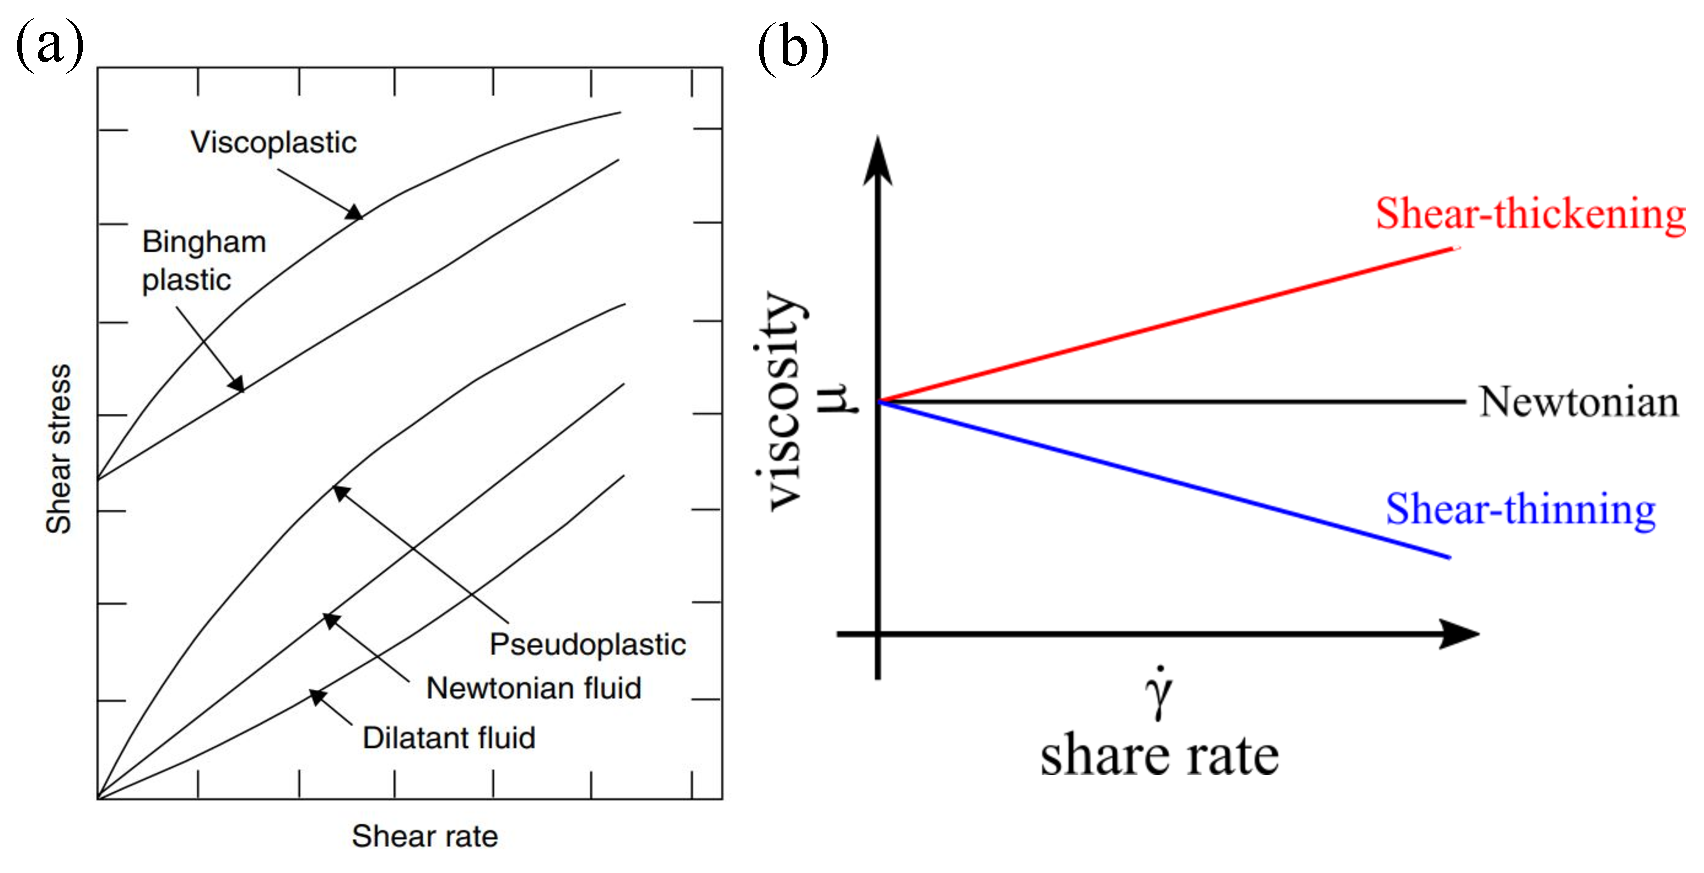
\includegraphics[width=1\textwidth]{1-Background/shea-thining.eps}
    \caption{(a) Qualitative flow curves for different types of non-Newtonian fluids\cite{ref:1}. (b)Classifications of non-Newtonian power-law fluid.}
    \label{fig:1-fluid-curve}
\end{figure}
\begin{figure}[ht]
    \begin{center}
        \includegraphics[width=12.0cm,clip]{1-Background/4-sinking.png}
        \caption{Sinking dynamics for different intruder-sizes and for different vibration intensities $\Gamma$. (a1) Depth$z$ versus time$t$ for $\dot{z}$ an intruder with radius of 4mm and (a2) for an intruder with radius of 7mm. (b1) Instantaneous velocity versus sinking depth $z$ obtained from (a1) and (b2) from (a2). The black lines correspond to the solutions fitted in the quasi-steady regime\cite{ref:6}.}
        \label{fig:4-sinking}
    \end{center}
\end{figure}
\newpage
\subsection{研究目的}

先行研究\cite{ref:8}において,超音波照射された擬塑性流体中を落下する球の高速化の要因として,音響境界層内部における粘度低下と,音響境界層の形成が関係していることが提案されている.また,高速化が弾性によって抑制されることが示唆されている.しかし,調査された流体や落下球の種類,径は限定的であり,弾性が高速化を抑制することは検証が十分ではない.落下球の密度や濃度密度を大きく変化させることで,球の周囲に生じる応力を変化させ,粘性と弾性それぞれ影響を明らかにすることができる.

本研究で用いた試験溶液では,球の落下による運動が高速の場合,粘性による影響が支配的であり,低速の場合は弾性による影響が支配的となる.落下球の終端速度を変化させることで粘性が支配的な場合と弾性が支配的な場合に分けて,超音波照射による高速化への影響を調査した.そこで,流体物性,落下物体の密度,落下球の径をより大きく変化させ実験を行った.超音波照射された擬塑性流体中を落下する球の高速化に対する粘弾性両方の影響を明らかにすることを目的とする.

\newpage
\chapter{実験方法}
\section{概要}
本実験では,0.5,1wt.\% ポリアクリルアミド(PAA)溶液(三菱ケミカル,AP805C)を擬塑性流体としてそれぞれ用いた.また,対照実験として水道水も用いた.作製したPAA溶液が適切なものであるか評価を行うため,非ニュートン流体における指標の一つとなる粘度の計測を行った.続いて,擬塑性流体に対する超音波照射による影響の密度依存性を調べるため,様々な落下球を用いて球落下実験行った.

\section{粘度計測}
粘度計測における計測機器の模式図を\ref{fig:viscosity}に示す.ステージと回転する円錐回転子の間に存在する試料によって付加されるトルクを計測することで粘度の計測を行う.粘度のせん断速度依存性を確認することで生成した溶液の性質の確認を行った.なお、計測範囲の都合上、水道水では

\begin{center}
    \begin{figure}[h]
        \includegraphics[clip,width=8.0cm]{2-Methods/Viscosity-Measurement.png}
        \caption{Viscosity measurement method.}
        \label{fig:viscosity}
    \end{figure}
\end{center}

\section{球落下実験}

使用した実験装置の概略図を\ref{device}に示す.外寸において高さ255mm,幅50mm,奥行き50mm,厚さ5mmの矩形アクリル水槽に試験溶液を満たした.その上に落下球把持用のピックアップツールをマグネットベースによって固定した.
% TODO:水槽外寸計測
\begin{center}
    \begin{figure}[H]
        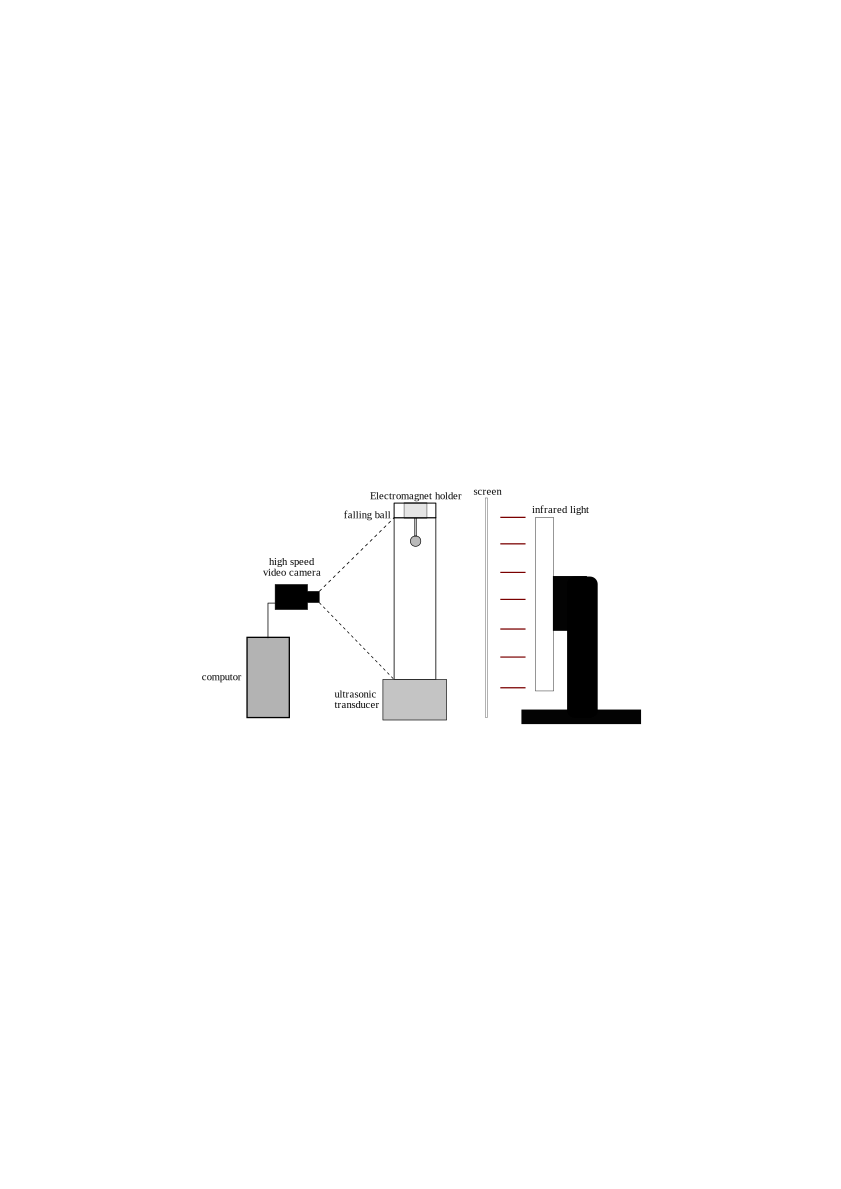
\includegraphics[clip,width=15.0cm]{2-Methods/device.png}
        \caption{Schematic view of the experimental apparatus.}
        \label{fig:device}
    \end{figure}
\end{center}

\newpage
\subsection{解析方法}
ハイスピードカメラを用いて落下球が落下する様子をbmp形式の連続画像として撮影すると,Fig\ref{fig:expPhoto}(a) に示すように,落下球以外にも電磁石や水槽壁面が映ってしまう.この画像から,落下球を検出するためにHough変換を用いた.Hough変換は任意の幾何形状の輪郭線に対して,特徴点を一定数以上通る曲線を検出する手法である.本実験では背景処理とSobel filterを用いて,球の輪郭画像を得た.
\subsubsection{背景処理とSobel filter}
上述のように,Hough変換の前処理として,背景処理とSobel filterの処理を行った.撮影した連続画像から得た背景処理画像をFig\ref{fig:expPhoto}(b) に示す.背景処理では,画像輝度値の平均値を計算しそれぞれの画像との差分を取った.これにより,移動を伴う球抽出できる.続いて,背景処理画像にSobel filterを適用した.Sobel filter処理後の画像をFig\ref{fig:expPhoto}(c) に示す.Sobel filterとは,輪郭抽出を行うフィルタ処理である.ある任意の画素を中心とした9つの輝度値に対し,Fig\ref{fig:sobel}(a)(b)に示す係数をそれぞれ乗算し合計した後,絶対値をとる.Fig\ref{fig:sobel}(a)により$y$軸方向の輪郭を,Fig\ref{fig:sobel}(b)により$x$軸方向の輪郭を強調する.Fig\ref{fig:sobel}(a)(b)それぞれによって,フィルタ処理された9つの輝度値に対する乗算の合計値を2乗し,足し合わせた後に平方することで平均をとった.これにより,落下球の輪郭を明確にした.

\begin{figure}[h]
    \centering
    \includegraphics[width=4.0cm,clip]{2-Methods/exp-img.png}
    \caption{(a) Original image, (b) Image used by background processing and, (c) Image used by Sobel filter.}
    \label{fig:expPhoto}
\end{figure}

\begin{figure}[h]
    \centering
    \includegraphics[width=7.0cm,clip]{2-Methods/sobel-filter.png}
    \caption{(a) Horizonal (b) Vertical Sobel filter.}
    \label{fig:sobel}
\end{figure}

\newpage

\subsubsection{Hough変換による円の検出}
背景処理とSobel filter処理を行った画像(Fig\ref{fig:expPhoto}(c))に,Hough変換を適用し円を検出した.検出手順は,以下に示す通りである.円は中心座標と半径により一意に定まる.このことより,円の中心座標 ($x_c$, $y_c$) ,半径$r$ による1つの円$D$ ($x_c$, $y_c$, $r$) に関して考えると,Fig\ref{fig:hough}に示すように画像内における任意の座標 ($x$, $y$) を通る円は無数に存在する.3つの円の中心座標$C_1$,$C_2$,$C_3$と座標 ($x$, $y$) から円の半径$r$が計算される.無数に存在する座標 ($x, $y) を通る円の座標Dに座標 ($x$, $y$) の輝度値を加算する.この処理を画像内全ての画素に対して行う.本実験におけるHough変換では輝度値の合計が最大となる座標$D$から球の中心座標及び半径を決定した.この中心座標の時間変化より,球の落下速度を計算した.

\begin{figure}[h]
    \centering
    \includegraphics[width=7.0cm,clip]{2-Methods/hough.PNG}
    \caption{Outline of Hough transform.}
    \label{fig:hough}
\end{figure}

\clearpage
\section{溶液物性および圧力場の確認}
\subsection{粘度 計測結果}
球落下実験を行う試験溶液として,異なる質量濃度のPAA溶液を製作した.この製作した溶液の粘度特性を得るため,粘度計を用いて計測を行った.なお,溶媒中の溶質が不均一な状態や,混合時に混入する気泡が存在する状態では,溶液の粘度が正しく計測できない.十分な溶質拡散や脱泡のために時間を要するため,粘度計測は溶液作製直後ではなく,1週間後に行った.それぞれの試料に対し,円錐回転子の回転数を変化させることでせん断速度を変化させ,粘度を各5回計測を行いその平均を求めた.

水道水の粘度計測結果をFig.\ref{fig:vis}(a)に示す.なお,縦軸は粘度,横軸はせん断速度を表す.第2.2節においても示したが,コーンロータの回転速度に応じて,液体のせん断速度を変化させた.その結果,粘度は1.1mPa$\cdot$sでほぼ一定となっていた.これは,水がニュートン流体であり,粘度を比例係数とした速度勾配とせん断応力の比例関係となっているためであると考えられる.また,理科年表\cite{理科年表}によると,水道水の粘度は20℃で1.0mPa$\cdot$sとなっている.これにより,適切に粘度計測が行えていると考えられる.

水道水の場合と同様にPAA溶液の粘度計測を行った結果をFig.\ref{fig:vis}(b)に示す.なお,縦軸は粘度の対数,横軸はせん断速度の対数を表す.ここで,粘度$\mu$はせん断速度$\dot{\gamma}$に対して,粘度定数 $k$,指数$n$を用い Power-law modelに従うものとすると,次式で表される\cite{ref:1}.
\begin{eqnarray}
	\label{eq:power-low}
	\mu=k\cdot\dot{\gamma}^{n-1}.
\end{eqnarray}
式(\ref{eq:power-low})を用いて近似線計算を行った結果を,Table \ref{table:power-law}に示す.溶液の濃度が濃いほど,擬塑性を示す$n$は小さくなり,より擬塑性が強くなった.粘性を表す$k$は,濃度の上昇に伴い大きくなった.これらより,PAA濃度が高くなると,より擬塑性が強く,粘性が大きい流体となることが分かった.

\begin{figure}[ht]
	\centering
	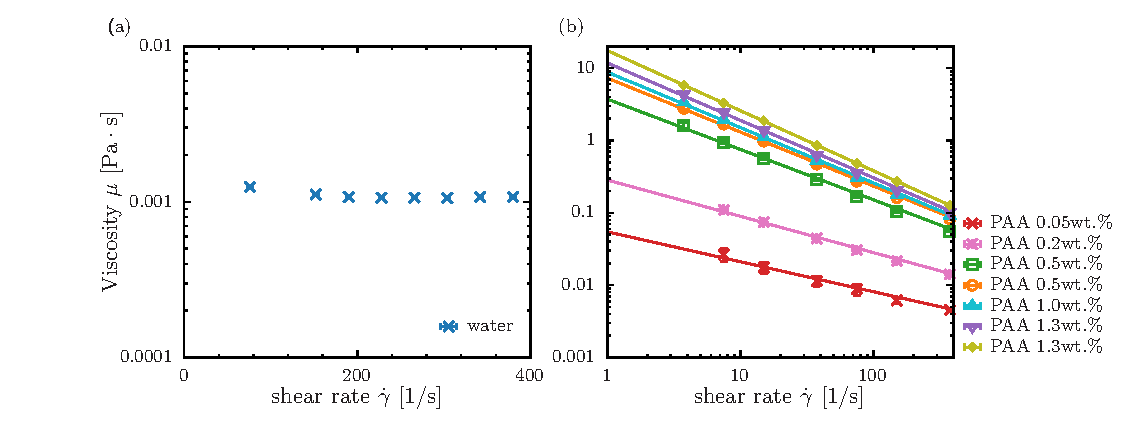
\includegraphics[width=15cm,clip]{3-Physical_Property/viscosity.eps}
	\caption{Viscosity versus shear rate for (a) tap water, (b) PAA solution.}
	\label{fig:vis}
\end{figure}

\begin{table}[h]
	\centering
	\caption{Parameters $k$ and $n$ in the Power-law model for each PAA solution at each concentration.}
	\label{table:power-law}
	\begin{tabular}{c|c|c|c|c|c|c|c} \hline
		PAA[wt.\%] & 0.05  & 0.2  & 0.5  & 0.7  & 1.0  & 1.3  & 1.5  \\ \hline \hline
		$k$        & 0.054 & 0.28 & 3.7  & 7.3  & 8.8  & 12   & 18   \\ \hline
		$n$        & 0.59  & 0.50 & 0.30 & 0.25 & 0.23 & 0.21 & 0.17 \\ \hline
	\end{tabular}
\end{table}

\newpage

\subsection{弾性率 計測結果}
\label{sec:elasticity}

作製したPAA溶液の応力に対する弾性特性を計測するため,それぞれのPAA質量濃度における,貯蔵弾性率$G'$,損失弾性率$G''$の応力依存性を計測した.また,式(\ref{eq:loss_factor})より損失正接$\tan\left(\eta\right)$を求めた.計測結果をFig.\ref{fig:PAA-elast}に示す.印可する応力が小さい場合,損失正接が1より小さく弾性による影響が強かった.また,応力を大きくすると,損失正接が1より大きくなり粘性による影響が強くなった.これより,応力が小さい場合は弾性による影響が,大きい場合は粘性による影響が大きくなることが分かった.加えて,濃度が濃くなると,貯蔵弾性率,損失弾性率共に大きくなった.これより濃度が高くなると溶液の粘弾性が強くなることが分かった.

ここで,損失正接が1となる応力$\tau$を$\tau_0$と定義する.各質量濃度における,$\tau_0$を内挿によって求めた結果をTable.\ref{table:PAA-tau0}に示す.質量濃度が上昇すると,$\tau_0$が大きくなった.このことより,濃度の増加に伴い,弾性による影響が大きくなる事が分かった.

\begin{figure}[ht]
	\centering
	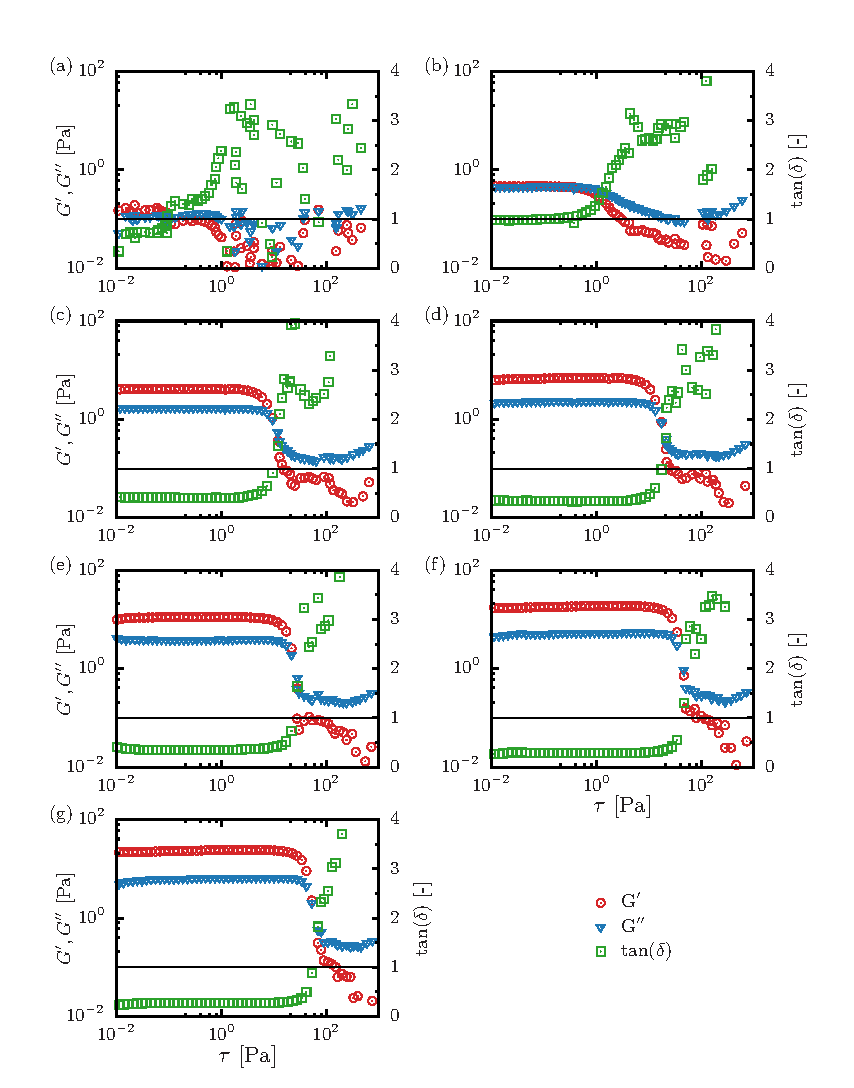
\includegraphics[width=1\textwidth]{3-Physical_Property/elastic_modulus.eps}
	\caption{Stress dependence of storage and loss elastic moduli for (a)0.05wt.\% (b)0.2wt.\% (c)0.5wt.\% (d)0.7wt.\% (e)1.0wt.\% (f)1.3wt.\% (g)1.5wt.\%.}
	\label{fig:PAA-elast}
\end{figure}

\begin{table}[h]
	\centering
	\caption{Relationship between concentration and $\tau_0$ for PAA solution.}
	\label{table:PAA-tau0}
	\begin{tabular}{c|c|c|c|c|c|c|c} \hline
		PAA[wt.\%]   & 0.05  & 0.2  & 0.5 & 0.7 & 1.0 & 1.3 & 1.5 \\ \hline \hline
		$\tau_0$[Pa] & 0.082 & 0.11 & 9.9 & 18  & 22  & 40  & 55  \\ \hline
	\end{tabular}
\end{table}

\clearpage

\subsection{圧力振幅 計測結果}

それぞれの質量濃度において,超音波圧力振幅の計測を行った.超音波圧力振幅の結果をFig.\ref{fig:pressure}に示す.縦軸は水槽底面からの高さ,横軸は圧力振幅である.この結果を元にTable \ref{table:press}に,圧力振幅$\Delta{}P$の$y$方向平均値$\Delta\overline{P}$を示す.水槽全体に圧力振幅が発生していることが確認された.

\begin{table}[h]
	\centering
	\caption{Averaged value of pressure amplitude.}
	\label{table:press}
	\begin{tabular}{c|c|c|c|c|c|c|c} \hline
		PAA[wt.\%]                & 0.05  & 0.2   & 0.5   & 0.7   & 1.0   & 1.3   & 1.5   \\ \hline \hline
		$\Delta\overline{P}$[kPa] & 112.2 & 129.7 & 143.8 & 150.3 & 156.2 & 199.5 & 191.1 \\ \hline
	\end{tabular}
\end{table}

\begin{figure}[ht]
	\centering
	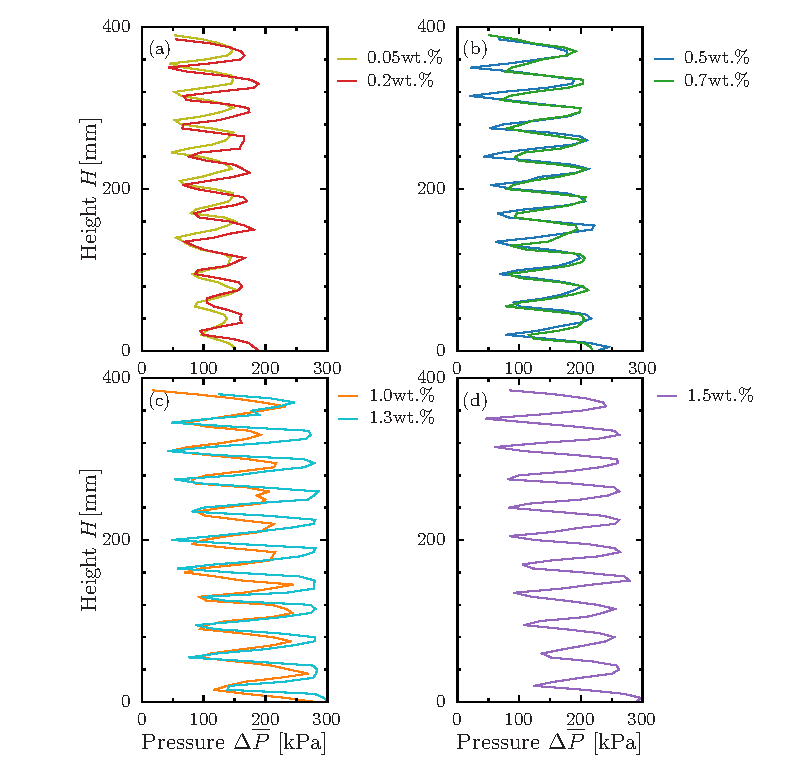
\includegraphics[width=0.9\textwidth]{3-Physical_Property/press.eps}
	\caption{Average pressure amplitude in (a)0.05wt.\% amd 0.2wt.\%, (b)0.5wt.\% and 0.7wt.\%, (c)1.0wt.\% and 1.3wt.\%, (d)1.5wt.\% PAA solution.}
	\label{fig:pressure}
\end{figure}

\newpage
\section{理論}
\ref{sec:exp-system}節に示した通り,本研究の系は超音波照射された擬塑性流体中を球が落下する系である.はじめに,擬塑性流体中を球が落下する理論を示すことで,球の終端速度の理論式を得る.続いて,球の落下によるせん断速度より,球の落下による応力を見積もる.最後に,超音波照射された擬塑性流体中を落下する球の高速化のメカニズムより,高速化の理論式を見積もる.

\subsection{擬塑性流体中における球の落下}
本研究の系において,代表速度,代表長さとして,落下球の終端速度$U_\text{T}$,球直径$D=2a$を選ぶ.Power-law model (式(\ref{eq:power-low}))が適用できる流体中おける粒子のレイノルズ数は次式で表される\cite{ref:1,ref:8-5}.
\begin{eqnarray}
    Re = \frac{\rho_1 \left(2a\right)^n U_T^{2-n}}{k} .
    \label{eq:re}
\end{eqnarray}
ここで,$\rho_1$は溶液密度である.今回の実験結果の代表例(鋼球,直径10mm,PAA1.0wt.\%)において,溶液密度$\rho_1\approx$1000kg/m$^3$,$2a=$0.01m,$U_T \approx$0.2m/s,$k=$8.8Pa$\cdot \text{s}^n$,$n=$0.23である.この条件より,式(\ref{eq:re})より$Re\approx$2.3と概算でき,粒子付近ではストークス流れに従うと考えられる.ゆえに,慣性に比べて粘性が支配的であると考えられる.

超音波の伝播に関して,音波の圧力変動の時間スケールは$O\left(10^{-5}\right)$sである.一方で,球の落下現象は$O\left(10^{-2}\right)$m,$O\left(10^{0}\right)$sとなり,圧力変動の時間スケールは非常に短い.球の落下に関しては,落下時間スケールで粗視化した平均的な挙動に着目する.球周囲に存在する非圧縮性流体の単位体積の運動方程式について考える.球によって誘起される応力テンソルを$\bm{\sigma}$,流体の密度を$\rho$,s周囲流体の速度ベクトルを$\bm{v}$,体積力を$\bm{X}$とすると,
\begin{eqnarray}
    \rho \frac{D\bm{v}}{Dt} = \bm{X} + \nabla \cdot \bm{\sigma} ,
    \label{eq:undou}
\end{eqnarray}
となる.また,非圧縮性流体を仮定しているため連続の式が成り立つ.
\begin{eqnarray}
    \nabla \cdot \bm{v} = 0 .
    \label{eq:renzoku}
\end{eqnarray}
粒子重心位置から見た移動座標系では,式(\ref{eq:undou})の左辺が,
\begin{eqnarray}
    \frac{D\bm{v}}{Dt} = \frac{\partial \bm{v}}{\partial t} + \left(\bm{v} - \bm{U}_T \cdot \nabla \right) \bm{v} ,
    \label{eq:nabie}
\end{eqnarray}
と展開できる.流れは十分に発達し,定常状態であると仮定することで,式(\ref{eq:nabie})の右辺第1項の時間微分項は0となる.低レイノルズ数かつStokes近似を用いることにより,慣性項は粘性項より十分に小さいと仮定することができる.これにより,式(\ref{eq:nabie})の右辺第2項の慣性項は無視することができる.加えて,粒子周囲流体には密度差がないため,静水圧分を除いた圧力を使って応力${\bm \sigma}$と書くと,体積力${\bm X}$は0となる.これらより,式(\ref{eq:undou}), (\ref{eq:nabie})を用いると,
\begin{eqnarray}
    \nabla \cdot \bm{\sigma} = 0 ,
    \label{eq:sigma-}
\end{eqnarray}
といった関係が導かれる.

ある球体領域において,ガウスの発散定理より,
\begin{eqnarray}
    \int_S{\bm{\sigma \cdot \bm{n}}}dS = \int_V{\nabla \cdot \bm{\sigma}}dV ,
    \label{eq:gaussian}
\end{eqnarray}
といった関係が成り立つ.ここで,$\bm{n}$は球領域表面に対する法線ベクトル,$S$は球の表面積,$V$は球の体積を表す.式(\ref{eq:sigma-})より,式(\ref{eq:gaussian})の右辺は0である.式(\ref{eq:sigma-}),(\ref{eq:gaussian})は任意の流体体積に関して成り立つため,球の表面($r = a$)と球外部の任意の領域($r > a$)において,以下の関係が成り立つ.
\begin{eqnarray}
    \int_{r=a}\bm{\sigma}\cdot\bm{e}_r dS=\int_r\bm{\sigma}\cdot\bm{e}_r dS .
    \label{eq:inte}
\end{eqnarray}
ここで,$\bm{n} = \bm{e}_r$とする.この式は,任意の領域において,面積力が釣り合うことを示す.$r = a$における時間平均応力を$\langle\sigma\rangle_a$,$r$における時間平均応力を$\langle\sigma\rangle_r$とそれぞれする.球の表面積$S=4\pi r^2$であるので,式(\ref{eq:inte})は,
\begin{eqnarray}
    4\pi a^2\langle\sigma\rangle_a = 4\pi r^2\langle\sigma\rangle_r ,
    \label{eq:sigma1}
\end{eqnarray}
となる.球表面において,球の体積力と表面力は釣り合うので,
\begin{eqnarray}
    4\pi a^2\langle\sigma\rangle_a = \frac{4}{3} \pi a^3 \Delta \rho g ,
    \label{eq:sigma2}
\end{eqnarray}
となる.ここで,球と流体の密度差$\Delta \rho$,重力加速度$g$である.式(\ref{eq:sigma1}),(\ref{eq:sigma2})より,
\begin{eqnarray}
    \langle\sigma\rangle_r = \frac{a^3\Delta\rho g}{3r^2} ,
\end{eqnarray}
となる.低レイノルズ数で粘性項が支配的であるため,
\begin{eqnarray}
    \langle\sigma\rangle_r \sim \mu \dot{\gamma} ,
    \label{eq:sigma3}
\end{eqnarray}
と概算することができる.Power-law modelが適用できる領域での議論を行っているため,式(\ref{eq:power-low}),(\ref{eq:sigma3})より,
\begin{eqnarray}
    \dot{\gamma} \sim \left(\frac{a^3\Delta\rho g}{3r^2 k}\right)^{\frac{1}{n}} ,
    \label{eq:gamma_abs}
\end{eqnarray}
と概算される.この系において,エネルギー散逸に関して考える.位置エネルギーと粘性によるエネルギー散逸が釣り合うため,単位時間あたりに系全体が失うエネルギーバランスより,以下の式が成立する.
\begin{eqnarray}
    \int_{r>a}\bar{\epsilon}dV = 4 \pi \int^\infty_a \bar{\epsilon}r^2 dr = \frac{4}{3}\pi a^3\Delta\rho g U_T ,
    \label{eq:eg}
\end{eqnarray}
ここで,$U_T$は球の終端速度,$\bar{\epsilon}$は時間平均された単位体積当たりのエネルギー散逸である.また,粘性散逸$\bar{\epsilon}$は,以下の様に概算される.
\begin{eqnarray}
    \bar{\epsilon} \sim \langle\sigma\rangle_r\dot{\gamma} \sim \mu \dot{\gamma}^2 \sim \frac{\langle\sigma\rangle_r^2}{\mu} ,
    \label{eq:eps}
\end{eqnarray}
式(\ref{eq:sigma3}),(\ref{eq:eg}),(\ref{eq:eps})より,終端速度は
\begin{eqnarray}
    U_T \sim \frac{a^3\Delta\rho g}{3}\int_a^\infty\frac{dr}{\mu r^2} ,
    \label{eq:UT0}
\end{eqnarray}
と見積もられる.式(\ref{eq:power-low}),(\ref{eq:gamma_abs}),(\ref{eq:UT0})より,終端速度は下記の様に書き直される.
\begin{eqnarray}
    U_T \sim \frac{a^3\Delta\rho g}{3}  \int^{\infty}_{a} \frac{dr}{\mu r^2} \sim \left(\frac{\Delta \rho g}{3k}\right)^{\frac{1}{n}}\frac{n}{2-n}a^{\frac{n+1}{n}} .
    \label{eq:UT}
\end{eqnarray}

\subsection{擬塑性流体中における球の落下による応力}
擬塑性流体中を落下する球の終端速度を$U_\text{T}$とする.,球の終端速度$U_\text{T}$と半径$a$を用いて,
\begin{eqnarray}
    \dot{\gamma} \sim \frac{U_\text{T}}{a},
    \label{eq:UTgamma}
\end{eqnarray}
と見積もられる.球の落下による粘度$\mu_\text{U}$は,式(\ref{eq:power-low})のPower-law modelより,
\begin{eqnarray}
    \mu_\text{U} \sim k \left(\frac{U_\text{T}}{a}\right)^{n-1} ,
    \label{eq:muU}
\end{eqnarray}
と見積もることができる.これより,式(\ref{eq:sigma3})より球の落下による応力$\tau_\text{U}$は,
\begin{eqnarray}
    \tau_\text{U} \sim k \left(\frac{U_\text{T}}{a}\right)^n ,
    \label{eq:tauU}
\end{eqnarray}
と見積もられる.

\subsection{超音波照射に伴う球の高速化}
\label{sec:UTdiff}
超音波照射された本研究の系における,落下球の高速化に関して考える.音響境界層における,せん断速度の代表値は次のように概算される.
\begin{eqnarray}
    \dot{\gamma} \sim \frac{u}{\delta} .
    \label{eq:abl-delta}
\end{eqnarray}
ここで,$u$は音波によって加振される流体粒子速度,$\delta$は音響境界層厚さを表す.

流体粒子速度$u$に関して,球の落下方向を$z$とすると運動方程式は次式となる.
\begin{eqnarray}
    \frac{\partial u}{\partial t} + \frac{1}{\rho_1}\frac{\partial P}{\partial z} = 0 .
    \label{eq:newton-1}
\end{eqnarray}
ここで,$t$は時刻,$P$は圧力である.また,連続の式は圧縮性流体と仮定すると以下の式となる.
\begin{eqnarray}
    \frac{\partial u}{\partial z} + \frac{1}{\rho_1 c^2}\frac{\partial P}{\partial t} = 0 .
\end{eqnarray}
音波の周波数は一定であり,容器内の圧力変化は音波に依存するので,以下の式の近似を用いる.
\begin{eqnarray}
    \frac{\partial u}{\partial t} &\sim& uf ,\label{eq:1-1}\\
    \partial P &\sim& \Delta P ,\label{eq:1-2}\\
    \partial z &\sim& \lambda .\label{eq:1-3}
\end{eqnarray}
ここで,$\Delta P$は音響圧,$\lambda$は超音波の波長である.式(\ref{eq:1-1}),(\ref{eq:1-2}),(\ref{eq:1-3})を用いて,式(\ref{eq:newton-1})の近似を行うと次式のようになる.
\begin{eqnarray}
    uf \sim \frac{\Delta P}{\rho_1 \lambda} .
    \label{eq:u-1}
\end{eqnarray}
周波数$f$,波長$\lambda$,音速$c$の関係から式(\ref{eq:u-1})を書き換えると次式となる.
\begin{eqnarray}
    u \sim \frac{\Delta P}{\rho_1 c} .
\end{eqnarray}

式(\ref{eq:abl-delta})より,Power-law model(式(\ref{eq:power-low}))を適用すると,音響境界層粘度$\mu_{ABL}$は次式の様に見積もられる.
\begin{eqnarray}
    \mu_{ABL} \sim k\left(\frac{u}{\delta}\right)^{n-1} ,
    \label{eq:muABL}
\end{eqnarray}
よって,音響境界層厚さ$\delta$は,
\begin{eqnarray}
    \delta \sim \sqrt{\frac{\mu_{ABL}}{\pi \rho_h f}} ,
    \label{eq:delta2}
\end{eqnarray}
と見積もられる\cite{deshpande2001vibrational,wiklund2012acoustofluidics}.ここで,周波数$f$である.よって,式(\ref{eq:delta2})を式(\ref{eq:muABL})に代入すると,次のように表される.
\begin{eqnarray}
    \delta \sim \left(\frac{k\left(\Delta P\right)^{n-1}}{\pi \rho^n_1 c^{n-1} f}\right)^{\frac{1}{n+1}} .
    \label{eq:delta}
\end{eqnarray}
ここで,音速$c$である.音響境界層粘度$\mu_{ABL}$とすると超音波照射下における終端速度$U_\text{ON}$は,式(\ref{eq:UT})より,
\begin{eqnarray}
    U_\text{ON} \sim \frac{a^3\Delta\rho g}{3}  \int^{\infty}_{a} \frac{dr}{\mu_{ABL} r^2} \sim \frac{a\Delta \rho \delta g}{3\mu_{ABL}} ,
    \label{eq:U_ABL}
\end{eqnarray}
と見積もられる.終端速度$U_T$における,粘度$\mu_U$とする.式(\ref{eq:UT}),(\ref{eq:U_ABL})より,超音波照射の有無による終端速度比は,
\begin{eqnarray}
    \frac{U_\text{on}}{U_\text{off}}=\frac{U_\text{ON}}{U_T} \sim \frac{\mu_U}{\mu_{ABL}}\frac{\delta}{a} ,
    \label{eq:Udiff}
\end{eqnarray}
と表される.

\newpage
\section{球密度による影響}

% //TODO:終端速度と高速化比を示す(横軸密度,質量濃度ごと)

落下させる球の密度を変化させた結果を,\ref{sec:expData}に示す.この結果より,それぞれの質量濃度における終端速度,高速化を求めると

球の落下速度の終端速度

式(\ref{eq:UdiffRho2})より,
\clearpage
\section{高速化に対する溶液濃度の影響}
\label{sec:concentration}
超音波照射による擬塑性流体中の落下球の高速化に対する溶液濃度の影響を調べる.実験条件をTable.\ref{table:exp-conditions}に示す.式(\ref{eq:Udiff})より,落下球高速化は球径の影響を受けることが示唆される.しかし,本実験条件では,球径の差が5\%程度にとどまることから,球径は同一として考える.

PAA溶液濃度と終端速度の関係をFig\ref{fig:concentrationUT}に示す.溶液濃度が高くなると,終端速度が遅くなる.超音波照射の有無による速度の比とPAA溶液濃度の関係を,Fig\ref{fig:concentrationUdiff}に示す.これらの結果より,縦軸を高速化度合,横軸を落下球の密度,溶液濃度の影響を考えた式(\ref{eq:UdiffRho})の右辺とした結果をFig\ref{fig:concentrationUdiff2}に示す.アルミニウム粒子では,濃度の上昇に伴い高速化度合が1.3程度となる正の相関が見られた.アルミナで粒子では,PAA濃度1.0wt.\%で高速化度合が1.2程度で最大となり,それ以上の濃度においては高速化度合が1に近づき,あまり高速化していない.ステンレス粒子では,濃度との相関が不明瞭であった.真鍮粒子では,PAA濃度0.7wt.\%の濃度で高速化度合が1.15程度で最大となった.これらをまとめた結果をFig\ref{fig:concentrationUdiffAll}に示す.超音波照射による速度比は,密度変化,粘度変化に対して弱い正の相関がみられた.高速化に対する溶液濃度の影響は存在するが,別の要因が生じているため弱い正の相関となったと考えられる.第\ref{sec:elasticity-discussion}章において,高速化への影響を与えていると考えられる,弾性による影響の議論を行う.

\begin{figure}[ht]
    \centering
    \includegraphics[width=0.8\textwidth]{./5-Results/concentrationUT.eps}
    \caption{Terminal velocity in PAA solution concentration.}
    \label{fig:concentrationUT}
\end{figure}

\begin{figure}[ht]
    \centering
    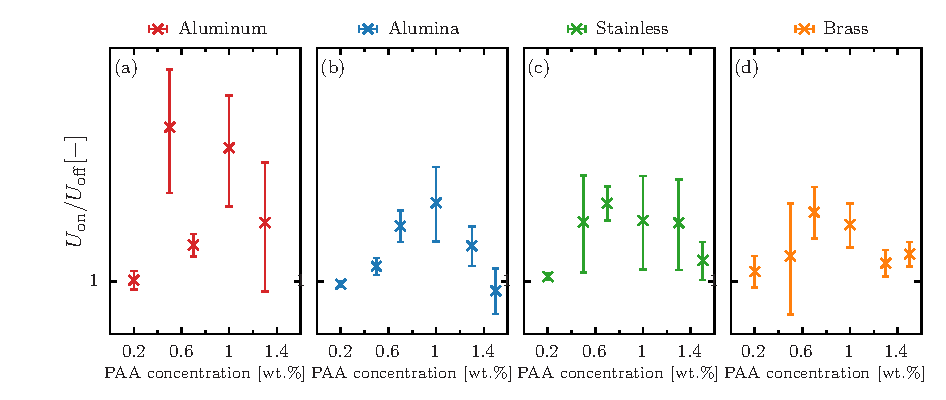
\includegraphics[width=1.0\textwidth]{./5-Results/concentrationUdiff.eps}
    \caption{Velocity ratio in PAA solution concentration (a)Aluminum, (b)Alumina, (c)Stainless, (d)Brass.}
    \label{fig:concentrationUdiff}
\end{figure}

\begin{figure}[ht]
    \centering
    \includegraphics[width=1.0\textwidth]{./5-Results/concentrationUdiff_each.eps}
    \caption{Velocity ratio in PAA solution concentration (a)Aluminum, (b)Alumina, (c)Stainless, (d)Brass.}
    \label{fig:concentrationUdiff2}
\end{figure}

\begin{figure}[ht]
    \centering
    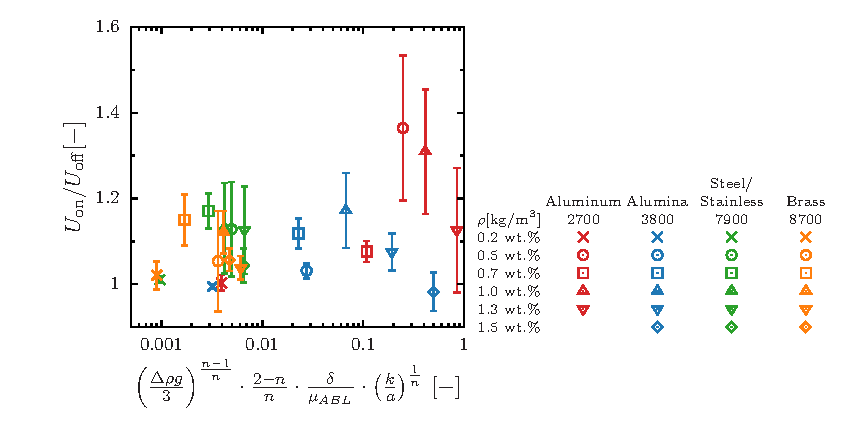
\includegraphics[width=0.7\textwidth]{./5-Results/concentrationUdiffAll.eps}
    \caption{Relationship between density, viscosity and terminal velocity.}
    \label{fig:concentrationUdiffAll}
\end{figure}
\clearpage
\section{球径による影響}
先行研究より拡張した領域における球径による影響を考えるため,直径を変化させた鋼球を用いて落下球実験を行った.実験条件は,Table.\ref{table:exp-conditions-dia}に示す通りである.それぞれの質量濃度の場合において検討を行う.

\subsection{PAA1.0wt.\%の場合}
PAA1.0wt.\%における球径変化の実験結果をFig.\ref{fig:diameter}に示す.その結果より,落下球の直径と終端速度の関係をFig.\ref{fig:diaUT}(a)に示す.落下球の直径が大きくなると,終端速度が指数関数的に高速化した.また,直径と超音波照射による高速化度合の関係をFig.\ref{fig:diaUT}(b)に示す.落下球の直径10mmをピークとして超音波照射による高速化が見られた.

これらより,式(\ref{eq:Udiff})を用いて整理した結果をFig.\ref{fig:muUdiff}に示す.Fig.\ref{fig:muUdiff}(a)においては先行研究である岩室\cite{ref:8}の実験結果全範囲を,Fig.\ref{fig:muUdiff}(b)においては今回の実験結果によって得られた範囲を拡大した結果を示す.落下球の直径10mm以上において,粘度比と音響境界層を球の半径で規格化した値は,超音波照射による球の高速化度合いに対して正の相関関係にあった.一方で先行研究において示されていた範囲においては,高速化が抑制され非常に小さな値となっていた.この要因として,先行研究である岩室\cite{ref:8}において弾性による影響が示唆されている.本研究\ref{sec:elasticity-discussion}章にて,それらの議論を行う.

\begin{figure}[ht]
    \centering
    \includegraphics[width=1\textwidth]{./5-Results/diaUT_Udiff.eps}
    \caption{Relationship between diameter and (a)terminal velocity, (b)velocity rato.}
    \label{fig:diaUT}
\end{figure}

\begin{figure}[ht]
    \centering
    \includegraphics[width=1\textwidth]{./5-Results/mu_Udiff.eps}
    \caption{Relationship between velocity rato and viscosity ratio, the acoustic boundary layer thickness, radius (a)with Iwamuro (2020), (b)without Iwamuro (2020).}
    \label{fig:muUdiff}
\end{figure}

\newpage

\subsection{PAA0.5wt.\%の場合}
PAA0.5wt.\%における球径変化の実験結果をFig.\ref{fig:diameter-0.5}に示す.その結果より,落下球の直径と終端速度の関係をFig.\ref{fig:diaUT0.5}(a)に示す.落下球の直径が大きくなると,PAA1wt.\%の場合と同様に終端速度が指数関数的に高速化した.また,直径と超音波照射による高速化度合いの関係をFig.\ref{fig:diaUT0.5}(b)に示す.PAA1wt.\%の場合と同様に落下球の直径10mmをピークとして超音波照射による高速化が見られた.

式(\ref{eq:Udiff})を用いて高速化度合を整理した結果をFig.\ref{fig:muUdiff0.5}に示す.落下球の直径が10mm以上において粘度比と音響境界層を球の半径で規格化した値は,超音波照射による球の高速化度合いに対して正の相関関係にあった.一方で,落下球の直径5mmは高速化度合いが非常に小さくなった.このことに関して,他の結果も含めて,本研究\ref{sec:viscosity},\ref{sec:elasticity-discussion}章にて,議論を行う.
\begin{figure}[ht]
    \centering
    \includegraphics[width=1\textwidth]{./5-Results/diameter-0.5/diaUT_Udiff.eps}
    \caption{Relationship between diameter and (a)terminal velocity, (b)velocity rato.}
    \label{fig:diaUT0.5}
\end{figure}

\begin{figure}[ht]
    \centering
    \includegraphics[width=0.8\textwidth]{./5-Results/diameter-0.5/mu_Udiff.eps}
    \caption{Relationship between velocity rato and viscosity ratio, the acoustic boundary layer thickness, radius.}
    \label{fig:muUdiff0.5}
\end{figure}

\clearpage

\subsection{PAA0.2,1.3wt.\%の場合}
PAA0.2,1.3wt.\%における球径変化の実験結果をFig.\ref{fig:diameter-0.2-1.3}に示す.その結果より,落下球の直径と終端速度の関係をFig.\ref{fig:diaUT0.2-1.3}(a)に示す.落下球の直径が大きくなると,他の質量濃度と同様に終端速度が高速化した.また,直径と超音波照射による高速化度合いの関係をFig.\ref{fig:diaUT0.2-1.3}(b)に示す.PAA0.2wt.\%において,あまり高速化は見られなかった.一方で,PAA1.3wt.\%において,落下球の直径が小さくなるとより高速化が見られた.

これらより,式(\ref{eq:Udiff})を用いて整理した結果をFig.\ref{fig:muUdiff0.2-1.3}に示す.粘度比と音響境界層厚さを球の半径で規格化した値は,超音波照射による球の高速化度合いに対して正の相関関係にあった.他の結果も含めて,本研究\ref{sec:viscosity},\ref{sec:elasticity-discussion}章にて,より詳しい議論を行う.

\begin{figure}[ht]
    \centering
    \includegraphics[width=0.9\textwidth]{./5-Results/diameter-0.2-1.3/diaUT_Udiff.eps}
    \caption{Relationship between diameter and (a)terminal velocity, (b)velocity rato.}
    \label{fig:diaUT0.2-1.3}
\end{figure}

\begin{figure}[ht]
    \centering
    \includegraphics[width=0.7\textwidth]{./5-Results/diameter-0.2-1.3/mu_Udiff.eps}
    \caption{Relationship between velocity rato and viscosity ratio, the acoustic boundary layer thickness, radius.}
    \label{fig:muUdiff0.2-1.3}
\end{figure}
\clearpage
\section{高速化に対する粘度比の影響}
\label{sec:viscosity}
超音波照射による球の高速化度合いは,粘度比$\mu_\text{U}/\mu_\text{ABL}$と音響境界層厚さ$\delta$を球の半径$a$で規格化した値の積で整理できると,先行研究\cite{ref:8}で示唆された.この手法を用いて,第\ref{sec:density},\ref{sec:concentration},\ref{sec:diameter}章に示した各実験結果を整理する.その結果をFig\ref{fig:viscosity_ratio}に示す.

横軸の値が0.2までの範囲において,超音波照射による高速化度合いは,粘度比と音響境界層厚さを球の半径で規格化した値の積に正に相関する.しかし,横軸の値が0.2を越えると,粘度比と音響境界層厚さを球の半径で規格化した値の積に相関が見られない.これより,超音波照射による球の高速化に関して,横軸の値が0.2までの範囲では式(\ref{eq:Udiff})が適用でき,それ以上では,式(\ref{eq:Udiff})が適用できないことが分かった.これは,落下球の半径が小さい場合,擬塑性流体の粘度が大きい場合,落下球と流体の密度差が小さい場合,横軸の値が大きくなる.この要因として,先行研究\cite{ref:8}において弾性による影響が示唆されている.第\ref{sec:elasticity-discussion}章で,それらを議論する.

\begin{figure}[ht]
    \centering
    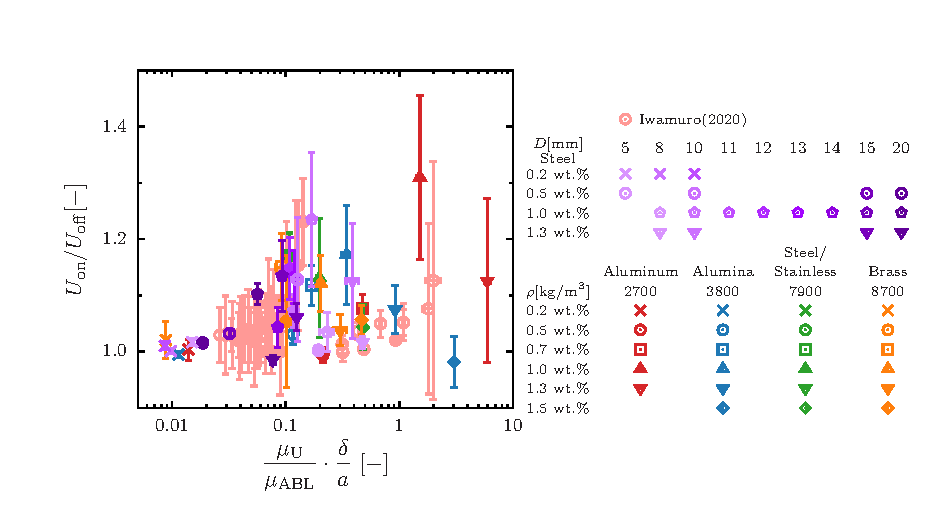
\includegraphics[width=1.0\textwidth]{5-Results/viscosity.eps}
    \caption{Relationship between velocity ratio and the inverse of the viscosity ratio multiplied by the thickness.}
    \label{fig:viscosity_ratio}
\end{figure}

\clearpage
\section{弾性による影響}

粘性による影響では説明が十分にできない
\clearpage
\newpage
\section{結言}
超音波照射された擬塑性流体中の落下球の高速化現象に関して,理論の妥当性を調査した.密度差,濃度,球径をパラメータとして実験した.以下に実験結果と得られた知見を示す.

\begin{itemize}
    \item 溶液と落下球の超音波照射による高速化度合と密度差の関係は,PAA濃度0.5,0.7wt.\%においては正の相関が,PAA濃度1.0wt.\%においては負の相関がみられた.理論では終端速度が遅くなる場合と,密度差が小さい場合に高速化が顕著となるものの,満たした場合はPAA濃度1.0wt.\%のみであった.これより,密度差以外による要因が大きいためと理論が適用できないと示唆される.
    \item 溶液の濃度を増加させた場合,落下球の終端速度は遅くなり,高速化がより顕著となる.しかし,濃度が高くなると高速化が抑制される.PAA溶液0.7-1.0wt.\%が高速化の極大となる.理論では溶液濃度が高い場合,高速化が顕著となると示される.これより,PAA濃度1.0wt.\%より溶液濃度が高い場合,理論が適用できないことが示唆された.
    \item PAA濃度1.0wt\%,落下球が鋼球の場合において直径を変化させた場合,直径10mmが高速化の極大となる.直径が10mmより大きい場合,高速化度合は粘度比と音響境界層厚さを落下球の半径で規格化した値の積と正の相関関係が見られる.一方で,球径が10mmより小さい場合,理論が適用できないことが示唆された.
    \item 本研究の実験条件において,高速化度合は粘度比と音響境界層厚さを球の半径で規格化した値の積が0.2以下において,正の相関がみられた.それ以上の範囲では高速化度合と粘度比と音響境界層厚さを球の半径で規格化した値との積に相関がみられなかった.応力比を用いて考えると,応力比1近傍にて高速化が顕著にみられ,それ以上では抑制されていた.これより,弾性影響が高速化を抑制することが分かった.
\end{itemize}

上記の結果から,超音波照射された擬塑性流体中の落下球の高速化現象に関して,理論が適用できる条件には限りがあることが分かった.弾性影響が無視できない粘弾性流体において,終端速度が遅い場合,理論が適用できないことが示唆された.弾性影響下で高速化現象を示すためには,弾性の影響を考慮した理論の構築が必要であると考えられる.
\newpage
\begin{appendices}
	\section{球落下実験 実験結果}
\label{sec:expData}

\subsection{密度・濃度による影響に関して}
本研究において,落下させる球の密度,擬塑性流体の質量濃度を変化させた.それぞれの質量濃度における,球の落下速度をFig.\ref{fig:0.05-0.2}-\ref{fig:1.5}に示す.横軸は経過時間$s$,縦軸は落下速度$m/s$である.

\begin{figure}[H]
    \centering
    \includegraphics[width=1.0\textwidth]{5-Results/0.05-0.2.eps}
    \caption{Velocity of a falling sphere made by (a)nylon in 0.05 wt.\% PAA solution, (b)aluminum, (c)alumina, (d)stainless,(e)brass in 0.2 wt.\% PAA solution.}
    \label{fig:0.05-0.2}
\end{figure}

\begin{figure}[H]
    \centering
    \includegraphics[width=1.0\textwidth]{5-Results/0.5-0.7.eps}
    \caption{Velocity of a falling sphere made by (a)aluminum, (b)alumina, (c)stainless,(d)brass in 0.5 wt.\% PAA solution, (e)aluminum, (f)alumina, (g)stainless,(h)brass in 0.7 wt.\% PAA solution.}
    \label{fig:0.5-0.7}
\end{figure}

\begin{figure}[H]
    \centering
    \includegraphics[width=1.0\textwidth]{5-Results/1.0-1.3.eps}
    \caption{Velocity of a falling sphere made by (a)aluminum, (b)alumina, (c)stainless,(d)brass in 1.0 wt.\% PAA solution, (e)aluminum, (f)alumina, (g)stainless,(h)brass in 1.3 wt.\% PAA solution.}
    \label{fig:1.0-1.3}
\end{figure}

\newpage

\begin{figure}[H]
    \centering
    \includegraphics[width=0.9\textwidth]{5-Results/1.5.eps}
    \caption{Velocity of a falling sphere made by (a)alumina, (b)stainless,(c)brass in 1.5 wt.\% PAA solution.}
    \label{fig:1.5}
\end{figure}

\subsection{球径による影響に関して}

球径を変化させた際の実験結果をFig.\ref{fig:diameter-0.5}-\ref{fig:diameter-0.2-1.3}に示す.横軸は経過時間$s$,縦軸は落下速度$m/s$である.

\begin{figure}[H]
    \centering
    \includegraphics[width=0.9\textwidth]{X-Appendix/diameter-0.5/diameter.eps}
    \caption{Velocity of a falling sphere in 0.5wt.\% PAA of (a)5mm, (b)15mm, (c)20mm.}
    \label{fig:diameter-0.5}
\end{figure}

\begin{figure}[H]
    \centering
    \includegraphics[width=1\textwidth]{X-Appendix/diameter/diameter.eps}
    \caption{Velocity of a falling sphere in 1.0wt.\% PAA of (a)8mm, (b)10mm, (c)11mm, (d)12mm, (e)13mm, (f)14mm, (g)15mm, (h)20mm.}
    \label{fig:diameter}
\end{figure}

\begin{figure}[H]
    \centering
    \includegraphics[width=1\textwidth]{X-Appendix/diameter-0.2_1.3/diameter.eps}
    \caption{Velocity of a falling sphere in 0.2wt.\% PAA of (a)5mm, (b)8mm, 1.3wt.\% PAA of (c)8mm, (d)15mm, (e)20mm.}
    \label{fig:diameter-0.2-1.3}
\end{figure}

	\clearpage
	% //TODO:真空ポンプを用いた場合と電磁石を用いた把持方法の比較文章を書く
\section{実験装置の改良による影響に関して}
\label{sec:reexp}

先行研究\cite{ref:8}において,電磁石を用いて,磁力によって球の把持を行っていた.本研究において,強磁性体以外の球の把持を行うため,真空ポンプを用いて吸引する手法に変更した.その把持手法の変化に伴う影響を議論する.

\subsection{実験装置}

電磁石を用いた実験装置をFig.\ref{fig:magnet_device}に示す.電磁石の磁力によって落下球の把持を行った.球を落下させるとき,電磁石への通電を切り,落下方向に力を加えて球を落下させた.また,本実験は先行研究と同様の条件で行うため,外寸において高さ248.5mm,幅47mm,奥行き47mm,厚さ3.5mmの矩形ガラス水槽で実験を行った.また,照射する超音波の周波数は39kHzとした.

\begin{figure}[ht]
    \centering
    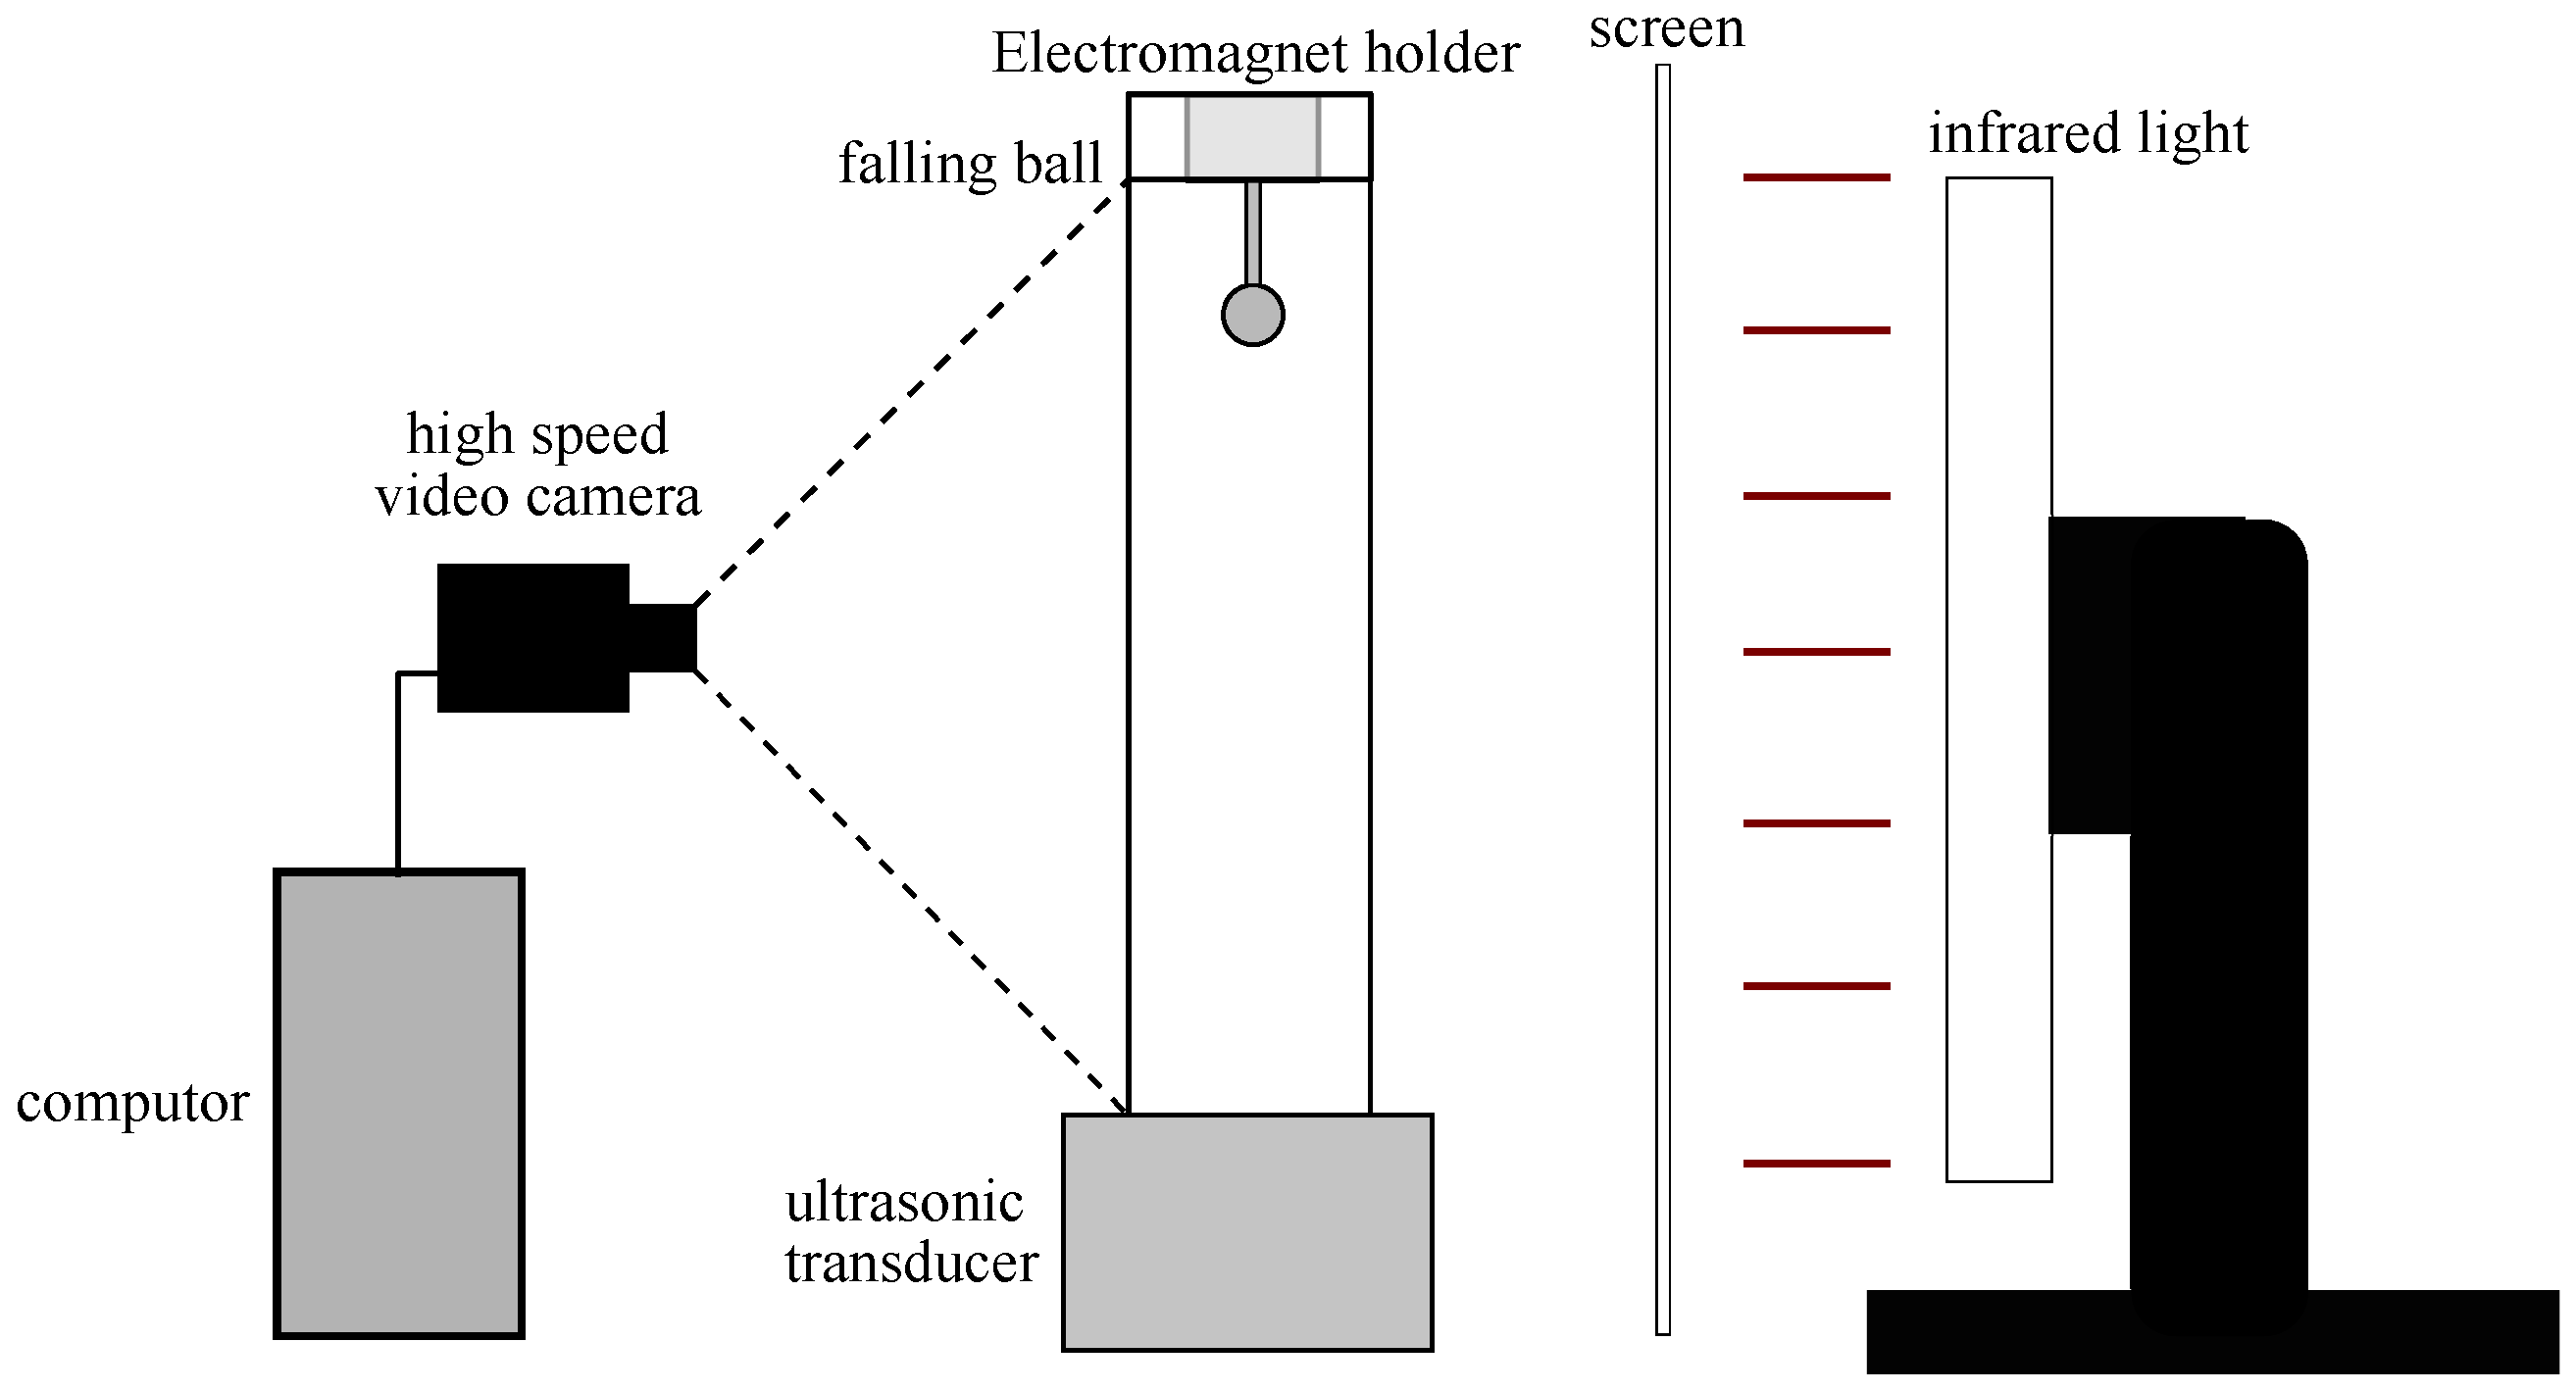
\includegraphics[width=0.95\textwidth]{X-Appendix/device/magnet_device.eps}
    \caption{Schematic view of the experimental apparatus by using electromagnet.}
    \label{fig:magnet_device}
\end{figure}

% Fig.\ref{fig:re-exp-vaccume}に真空ポンプを用いた把持方法における再現性の確認の実験結果を示す.縦軸は落下速度,横軸は落下開始時からの経過時間である.この再現性確認において,溶液の再作成から行った.終端速度に達するまでの経過はほぼ同様であった.一方で,終端速度は約10\%の誤差が生じた.これは,溶液の作製による誤差の影響を受けていると考えられる.

% \begin{figure}[ht]
%     \centering
%     \includegraphics[width=14cm,clip]{X-Appendix/reexp.png}
%     \caption{Falling velocity of a sphere in 1wt.\%PAA solution with and without ultrasound irradiation in tank A (reproducibility check).}
%     \label{fig:re-exp-vaccume}
% \end{figure}

\subsection{落下実験結果}

真空ポンプを用いて球を把持した場合と電磁石を用いて球を把持した場合の結果をFig\ref{fig:falling-A}に示す.縦軸は落下速度,横軸は落下開始時からの経過時間である.先行研究であるIwamuro \textit{et al}.\cite{ref:8}や電磁石を用いて球を把持した場合と比較し,超音波照射による高速化が顕著に現れなかった.また,落下開始時に電磁石を用いた場合はオーバーシュートが見られるが,真空ポンプを用いた場合はオーバーシュートが見られなかった.

\begin{figure}[ht]
    \centering
    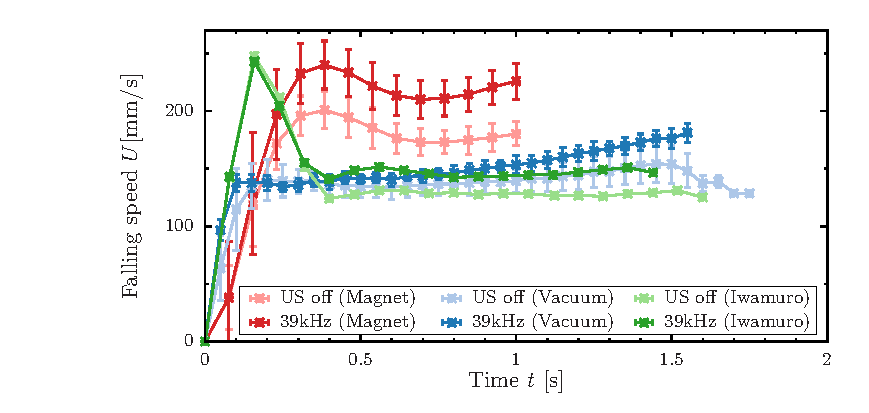
\includegraphics[width=1\textwidth]{./X-Appendix/magnet_vacuum/magnet_vacuum.eps}
    \caption{Falling speed of a sphere in 1wt.\%PAA solution with and without ultrasound irradiation.}
    \label{fig:falling-A}
\end{figure}


\subsection{落下開始時のオーバーシュートへの影響}
\label{sec:dis-de}

今回,球を把持する手法を,電磁石を用いて把持する方法から真空ポンプを用いて把持する方法に変化させた.この時,落下開始時0-0.3sにおける落下速度のオーバーシュートが,先行研究\cite{ref:8,ref:9}より小さくなった.落下開始時のオーバーシュートは弾性による影響によって生じる\cite{ref:12}.以下で,オーバーシュートが見られなくなった原因を,物質の流動性を表す$De$数より考える.$De$数が大きくなると,弾性的傾向が強くなり,$De$数が小さくなると,粘性的流動を表す.

$De$数は下記の様に緩和時間$\lambda$,代表時間$T$の比で表される.
\begin{equation}
    De = \frac{\lambda}{T} .
    \label{eq:De}
\end{equation}
代表時間$T$に関して,超音波照射を行っていない場合の球の落下条件においても考えるため,
\begin{equation}
    T = \frac{a}{U} ,
    \label{eq:T}
\end{equation}
となる.ここで,球の落下速度$U$,球の半径$a$である.また,緩和時間$\lambda$は,粘度$\mu$,貯蔵弾性率$G'$を用いて,
\begin{equation}
    \lambda \approx \frac{\mu}{G'} ,
    \label{eq:lamda}
\end{equation}
と見積もられる.緩和時間は変形の経過時間において,粘弾性流体が流体的挙動を示すか,固体的挙動を示すかの指標である\cite{ref:sakanishi}.粘度$\mu$に関して,落下球によるせん断領域における粘度となるため,式(\ref{eq:muU})の$\mu_\text{U}$を用いる.

これら式(\ref{eq:De}),(\ref{eq:T}),(\ref{eq:lamda}),(\ref{eq:muU})より,$De$数は,
\begin{equation}
    De \sim \frac{k}{G'} {\left(\frac{U}{a}\right)}^n ,
    \label{eq:De2}
\end{equation}
となり,粘度定数$k$,貯蔵弾性率$G'$,落下速度$U$,球の半径$a$によって見積もられる.

貯蔵弾性率$G'$[Pa]に関して,Fig.\ref{fig:PAA-elast}にて示した応力との関係性の結果を用いる.ここで応力$\tau$は,落下球によって生じた応力$\tau_\text{U}$を用いる.

Fig. \ref{fig:iwamuro-fall}に先行研究であるIwamuro \it{et al}.\cite{ref:8}の球径ごとの実験結果を示す.Fig.\ref{fig:falling-A}, \ref{fig:iwamuro-fall}それぞれの結果より,ピーク速度$U_{peak}$と終端速度$U_{ave}$を算出した.続いて,式(\ref{eq:tau-cal})を用いて,それぞれの速度における応力$\tau_{peak}$,$\tau_{ave}$の算出を行った.これら算出結果と先行研究の計測結果Fig.\ref{fig:iwamuro-G}より,貯蔵弾性率$G'$も求めた.これらの結果を,Table \ref{table:iwamuro}に示す.

また,式(\ref{eq:muU})を用いて,ピーク速度/終端速度それぞれの粘度$\mu_{peak}$,$\mu_\text{U}$を概算した.これらの粘度を式(\ref{eq:lamda})に代入し,それぞれの緩和時間$\lambda_{peak}$,$\lambda_{ave}$の算出を行った.そして,それらの緩和時間より,式(\ref{eq:De})を用いて,それぞれの$De$数,$De_{peak}$,$De_{ave}$を求めた.これらの結果を,Table \ref{table:iwamuro2}に示す.

Table \ref{table:iwamuro2}より,ピーク速度より求めた$De_{peak}$と,終端速度より求めた$De_{ave}$において,大きな差異が見られないことが分かった.以降,$De_{peak}$に関してのみ議論を行う.$De_{peak}$に関して,落下速度のオーバーシュート$U_{peak}/U_{ave}$との関係をFig.\ref{fig:De-overshoot}に示す.横軸は$De$数,縦軸は落下速度のオーバーシュート$U_{peak}/U_{ave}$である.この図より,$De$数とオーバーシュートには正の相関があり,$De$数が増加するとオーバーシュートも大きくなることが分かった.

\begin{table}[hbtp]
    \caption{Peak speed $U_{peak}$/ terminal speed $U_{ave}$, stress $\tau$, storage modulus $G'$ Calculation result.}
    \label{table:iwamuro}
    \centering
    \begin{tabular}{ccccccc}
        \hline
        \multirow{2}{*}{実験者}  & 球直径[mm] & ピーク速度[mm/s] & 終端速度[mm/s] & \multicolumn{2}{c}{応力[Pa]} & 貯蔵弾性率[Pa]        \\
                                 & $D=2a$     & $U_{peak}$       & $U_{ave}$      & $\tau_{peak}$                & $\tau_{ave}$   & $G'$ \\
        \hline \hline
        \multirow{8}{*}{Iwamuro} & 3          & 10.08            & 9.05           & 14.6                         & 14.2           & 8    \\
                                 & 4          & 23.2             & 19.4           & 16.5                         & 15.9           & 7    \\
                                 & 5          & 34.8             & 32.6           & 17.2                         & 17.0           & 6.7  \\
                                 & 6          & 46.3             & 54.8           & 17.6                         & 18.3           & 6.5  \\
                                 & 7          & 79.8             & 82             & 19.3                         & 19.4           & 5.5  \\
                                 & 8          & 130              & 113            & 20.9                         & 20.3           & 5    \\
                                 & 9          & 193              & 133            & 22.3                         & 20.5           & 4    \\
                                 & 10         & 256              & 168            & 23.2                         & 21.2           & 3.5  \\
        \hline \hline
        Niwa                     & 10         & 148              & 144            & 18.9                         & 18.7           & 6    \\
        \hline
    \end{tabular}
\end{table}
\begin{table}[hbtp]
    \caption{Viscosity $\mu$, Relaxation time $\lambda$, number of $De$ Calculation result.}
    \label{table:iwamuro2}
    \centering
    \begin{tabular}{ccccccccc}
        \hline
        \multirow{2}{*}{実験者}  & 球直径     & \multicolumn{2}{c}{粘度[Pa$\cdot$s]} & \multicolumn{2}{c}{緩和時間[s]} & \multicolumn{2}{c}{$De$数[-]}                                              \\
                                 & $D=2a$[mm] & $\mu_{peak}$                         & $\mu_{ave}$                     & $\lambda_{peak}$              & $\lambda_{ave}$ & $De_{peak}$ & $De_{ave}$ \\
        \hline \hline
        \multirow{8}{*}{Iwamuro} & 3          & 2.17                                 & 2.36                            & 0.27                          & 0.29            & 1.82        & 1.78       \\
                                 & 4          & 1.42                                 & 1.63                            & 0.20                          & 0.23            & 2.36        & 2.26       \\
                                 & 5          & 1.24                                 & 1.30                            & 0.18                          & 0.19            & 2.57        & 2.53       \\
                                 & 6          & 1.14                                 & 1.00                            & 0.18                          & 0.15            & 2.71        & 2.82       \\
                                 & 7          & 0.85                                 & 0.83                            & 0.15                          & 0.15            & 3.51        & 3.53       \\
                                 & 8          & 0.64                                 & 0.72                            & 0.13                          & 0.14            & 4.19        & 4.05       \\
                                 & 9          & 0.52                                 & 0.69                            & 0.13                          & 0.17            & 5.58        & 5.12       \\
                                 & 10         & 0.45                                 & 0.63                            & 0.13                          & 0.18            & 6.64        & 6.03       \\
        \hline \hline
        Niwa                     & 10         & 0.64                                 & 0.65                            & 0.11                          & 0.11            & 3.15        & 3.12       \\
        \hline
    \end{tabular}
\end{table}

\begin{figure}[ht]
    \begin{center}
        \includegraphics[width=13cm,clip]{X-Appendix/over_shoot/iwamuro-fall.png}
        \caption{Speed of a falling sphere in diameter of (a) 3 mm, (b) 4 mm, (c) 5 mm, (d) 6 mm, (e) 7 mm, (f) 8 mm, (g) 9 mm, (h) 10 mm in 1.0 wt.\% PAA solution with ultrasound fixed frequency at 27.4 kHz and $\Delta \bar{P} \approx$ 180 kPa\cite{ref:8}.}
        \label{fig:iwamuro-fall}
    \end{center}
\end{figure}

\begin{figure}[ht]
    \begin{center}
        \includegraphics[width=15cm,clip]{5-Results/De-overshoot.png}
        \caption{Relationship between overshoot $U_{peak}/U_{ave}$ and Deborah number $De$ for falling spheres.}
        \label{fig:De-overshoot}
    \end{center}
\end{figure}

\clearpage

\section{初速による影響に関して}

前節にて,実験装置の改良によってピーク速度が減少し,$De$が小さくなったことによってオーバーシュートが小さくなったことを示した.本節において,電磁石を用いて把持した場合,ピーク速度が大きくなった理由に関して考察を行う.電磁石を用いて球を把持した場合,電磁石へ落下方向に力を与えて落下を開始させている.この時,微小ではあるが落下開始時に初速が存在する.一方で真空ポンプを用いて球を把持した場合,吸着パッドを大気圧にすると球は落下する.この場合,球に力が加わらないため,初速は存在しない.このように初速の有無がオーバーシュートの変化に大きく関与していると考えられる.

初速の有無が与える影響に関して調査するため,真空ポンプを用いて球中心が液面より高さ$H=$5mmとなる地点で把持し,そこから球を落下させた.その結果をFig.\ref{fig:h-5}に示す.縦軸は落下速度,横軸は初速ありの場合は液面に球中心が入ったときを0s,初速なしの場合は落下開始時刻を0sとした時刻である.この条件において,初速は313[mm/s]となる.ピーク速度は440[mm/s]となり,初速を超えて加速した.これは初速と重力による加速が,粘性抵抗や浮力よりも大きく,弾性は遅れて発生するため,初速を超えて加速したと考えられる.

Iwamuro\cite{ref:9}の$a =$5[mm]における初速を推定する.この結果において,0.1sの時185[mm/s]であった.球の初速を$U_0$とすると,$U_0$の取りうる値の範囲は,0$\leqq U_0 \leqq$185[mm/s]となる.一方で,ピーク速度は256[mm/s]となり,オーバーシュートが見られた.これは,先述の初速を与えた結果と同様に弾性による影響が生じる前に初速や重力によって加速したためだと考えられる.

また,真空ポンプを用いた落下実験(niwa exp.)の$De$数は,先行研究の結果において球半径$3<a<3.5$[mm]の間における$De$数に相当した.電磁石を用いて把持した実験において,この球径においてオーバーシュートはあまり見られなかった.真空ポンプを用いた落下実験の場合,$De$数が小さくなった原因であるが,初速が存在しないため急激な速度変化とならず,ピーク速度$U_{peak}$が小さくなったためと考えられる.

よって,電磁石を用いて球を把持した場合は初速による影響がオーバーシュートとして現れるが,真空ポンプを用いて球を把持した場合は初速が非常に小さいためその影響を受けないということが分かった.

\begin{figure}[ht]
    \begin{center}
        \includegraphics[width=15cm,clip]{5-Results/h-5.png}
        \caption{Falling speed of a sphere in 1wt.\% PAA solution falling with initial speed.}
        \label{fig:h-5}
    \end{center}
\end{figure}
	\clearpage
	\input{X-Appendix/C-change_over_time.tex}
	\clearpage
	\section{溶液作製精度に関して}

溶液の作製精度の確認を行うため,0.95,1.00,1.05wt.\%のPAA溶液を作製した.それぞれの擬塑性流体に直径10mmの鋼球を落下させ,終端速度の変化,超音波照射による影響の変化の確認を行った.

\subsection{溶液の粘性特性に関して}
それぞれの溶液の特性を確認するため,粘度計を用いて粘度計測を行った.粘度計測を行った結果をFig.\ref{fig:95-105}に示す.比較のため,先行研究である岩室\cite{ref:8}とShiratori \it{et al}.\cite{ref:9}の計測結果も合わせて示す.濃度が薄いと粘度は低く,濃度が高いと粘度は高くなった.


\begin{figure}[ht]
    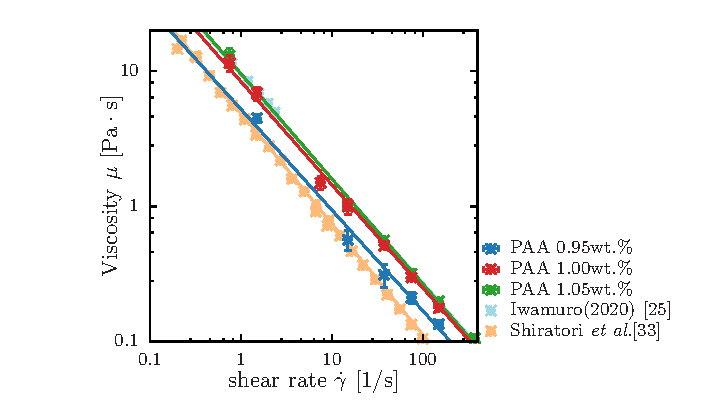
\includegraphics[width=1\textwidth]{X-Appendix/concentration/viscosity/viscosity.eps}
    \caption{Viscosity versus shear rate for PAA0.95,1.00,1.05wt.\%.}
    \label{fig:95-105}
\end{figure}

\subsection{溶液の作製精度による高速化への影響に関して}

ぞれぞれの質量濃度のPAA溶液に対し,落下球実験を行った.落下させた球は,鋼製の直径10mmの球である.

	\clearpage
	\section{落下間隔変化における高速化への寄与}
先行研究\cite{ref:8-5}にて,等間隔の時間で物体を落下させると,落下速度が一定になることが報告されている.これは,落下によって破壊された分子構造が回復するためだと考えられる.球の落下間隔を変化させると,PAA溶液の粘性弾性回復に対して影響を与えると考えられる.これらの落下速度,高速化への影響を調査するため,落下間隔を変化させた実験を行った.

落下間隔を5分,10分,20分と変化し,球を落下させた解析した結果をFig.\ref{fig:falling-interval}に示す.縦軸は落下速度,横軸は落下開始時からの経過時間である.それぞれの場合において,超音波照射による落下球の高速化は見られた.落下間隔と落下球の終端速度の関係をFig\ref{fig:falling-interval-diff}(a)に示す.縦軸は落下球の終端速度,横軸は落下間隔である.落下間隔を変化させた場合,落下間隔が5分と10分の場合に終端速度に大きな変化は生じなかった.一方で,落下間隔が20分の場合は終端速度の分散が小さくなった.これは,弾性回復が十分に行われたため,落下中の落下速度が一定に近くなったためだと考えられる.落下間隔と高速化度合の関係をFig\ref{fig:falling-interval-diff}(b)に示す.縦軸は高速化度合,横軸は落下間隔である.落下間隔を変化させた場合,超音波照射による高速化度合に対して大きな変化が見られなかった.また,粘度比と音響境界層を球の半径で規格化した値と高速化度合の関係をFig.\ref{fig:falling-interval-diff}(c)に示す.縦軸は高速化度合,横軸は粘度比と音響境界層を球の半径で規格化した値である.粘度比と音響境界層を球の半径で規格化した値は落下間隔を変化させた場合,あまり大きく変化しなかった.これは流体物性がほぼ同一であるためと考えられる.これらの結果より,今回の実験範囲ではあまり大きな変化が現れなかったことが分かった.
\begin{figure}[H]
    \centering
    \includegraphics[width=1\textwidth]{./X-Appendix/interval/interval.eps}
    \caption{Falling speed of a sphere in 1.0wt.\%PAA solution with and without ultrasound irradiation for the interval (a)5min, (b)10min, (c)20min.}
    \label{fig:falling-interval}
\end{figure}

\begin{figure}[H]
    \centering
    \includegraphics[width=1\textwidth]{./X-Appendix/interval/interval_cal.eps}
    \caption{ Relationship between (a)terminal velocity and interval, velocity ratio and (b) interval, (c)viscosity ratio.}
    \label{fig:falling-interval-diff}
\end{figure}

	%    \clearpage
	%    \section{落下手法の変化}

本文中における実験は,電磁石ホルダーを用いて鋼球を把持しているため,強磁性の材質の物体のみ把持することができる.
他の物質の物体を把持することのできる爪式ピッキングツールを用いて物体の把持を行い,球の落下試験を行った.
以下にその方法と結果を示す.

\subsection{実験方法}

今回,落下球の把持の方法を変化させただけであるので,実験装置の落下球把持の部分以外は先述の方法と同一である.

\subsubsection{実験装置}

実験装置の模式図をFig.\ref{fig:device2}に示す.先述の通り,電磁石ホルダーではなく,爪式ピックアップツールを用いて球の把持を行った.そして,ピックアップツールの開放を行うことで球を落下させた.それ以外に関しては,本文中の実験装置と同一である.

\begin{figure}[h]
    \centering
    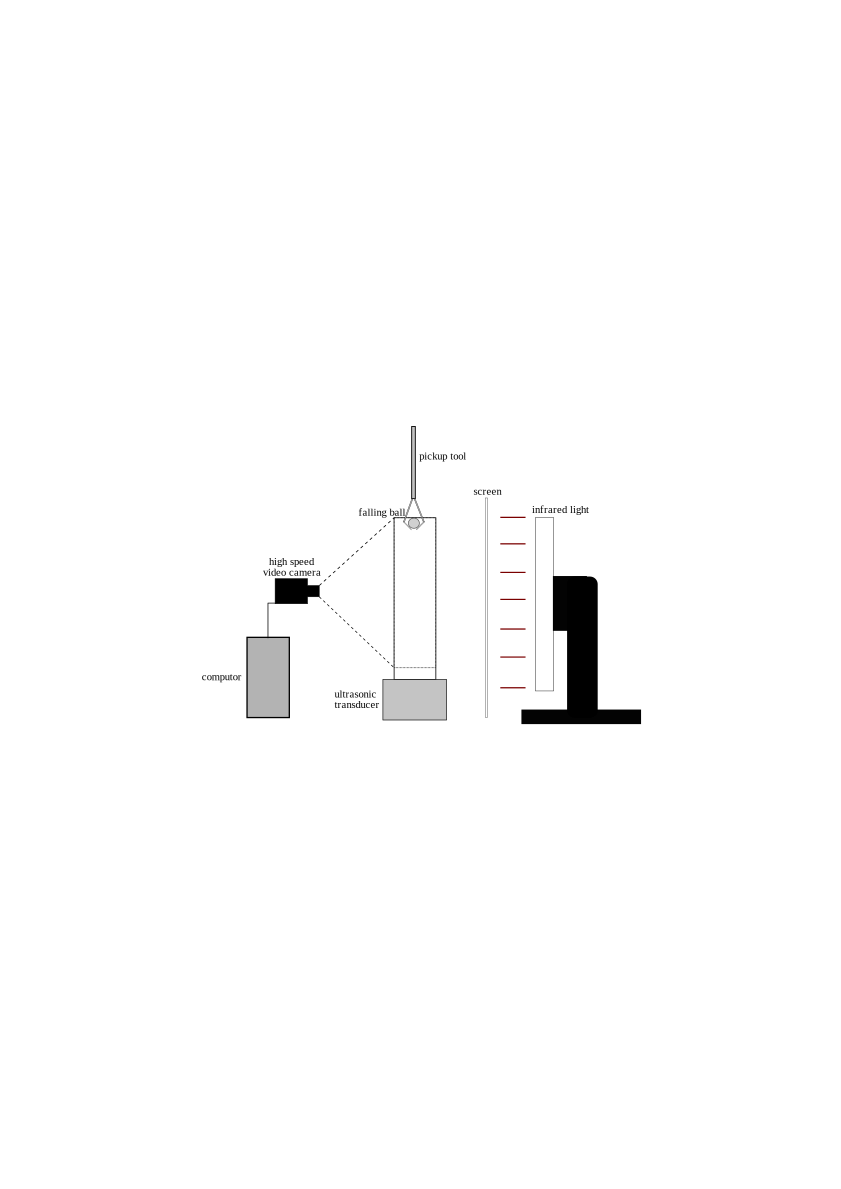
\includegraphics[clip,width=12.0cm]{X-Appendix/device.png}
    \caption{Schematic view of the experimental apparatus.}
    \label{fig:device2}
\end{figure}

\subsection{落下球 実験結果}

1wt.\%PAA溶液中における球の落下速度を解析した結果をFig.\ref{fig:1-1PAA-falling}に示す.縦軸は落下速度,横軸は落下開始時からの経過時間である.先述の電磁石ホルダを用いたFig.\ref{fig:1PAA-falling}とは異なり,超音波照射の有無において落下速度の高速化は見られなかった.一方で,先行研究であるIwamuro {\it et al.}\cite{ref:9}と同様に初めの加速後は減速し一定速度となった.

また,電磁石ホルダを用いた場合と同様に,超音波照射なしの状態における1から5試行目の結果をFig.\ref{fig:1-1PAA-falling1-5}に,6から10試行目の結果をFig.\ref{fig:1-1PAA-falling6-10}に示す.また,超音波照射ありの状態における1から5試行目の結果をFig.\ref{fig:1-1onPAA-falling1-5}に,6から10試行目の結果をFig.\ref{fig:1-1onPAA-falling6-10}に示す.これら試行ごとの結果において,先述のFig.\ref{fig:1PAA-falling1-5}-\ref{fig:1onPAA-falling6-10}の結果とは異なり落下速度のばらつきが非常に小さくなっていた.

\begin{figure}[ht]
    \centering
    \includegraphics[width=12cm,clip]{./X-Appendix/s1.png}
    \caption{Falling velocity of a sphere in 1wt.\%PAA solution with and without ultrasound irradiation.}
    \label{fig:1-1PAA-falling}
    \centering
    \includegraphics[width=12cm,clip]{X-Appendix/s1-0-1-5.png}
    \caption{Falling velocity of the sphere for each trial (\#1 to \#5) in 1wt.\%PAA solution without ultrasonic irradiation.}
    \label{fig:1-1PAA-falling1-5}
\end{figure}
\begin{figure}[ht]
    \centering
    \includegraphics[width=12cm,clip]{X-Appendix/s1-0-6-10.png}
    \caption{Falling velocity of the sphere for each trial (\#6 to \#10) in 1wt.\%PAA solution without ultrasonic irradiation.}
    \label{fig:1-1PAA-falling6-10}
    \centering
    \includegraphics[width=12cm,clip]{X-Appendix/s1-39-1-5.png}
    \caption{Falling velocity of the sphere for each trial (\#1 to \#5) in 1wt.\%PAA solution with ultrasonic irradiation.}
    \label{fig:1-1onPAA-falling1-5}
    \centering
    \includegraphics[width=12cm,clip]{X-Appendix/s1-39-6-10.png}
    \caption{Falling velocity of the sphere for each trial (\#6 to \#10) in 1wt.\%PAA solution with ultrasonic irradiation.}
    \label{fig:1-1onPAA-falling6-10}
\end{figure}

\subsection{考察}

電磁石ホルダを用いた把持方法と爪式ピッキングツールを用いた把持方法では試行ごとの落下速度の時間変化や超音波照射による高速化の有無において変化が見られた.以下に把持方法の変化による影響に関して検討を行う.

まず,電磁石ホルダを使用する場合,落下開始1分前に電源を切り,電磁石ホルダの把持力をゼロにする.しかし,落下させる対象の鋼球や溶液中に把持しているために存在する鋼製棒に磁性が残っている.また,落下球はPAA溶液中に存在するため浮力や粘弾性の影響を受ける.そのため落下開始時まで,把持している鋼製棒に接触したままとなっている.ここに,非常に弱い撃力を指で与え,落下させている.撃力による初速への影響
弾性によって減速が大きくなる可能性が存在する.

続いて,ピッキングツールを使用する場合に関して検討を行う.ピッキングホルダは球の把持を行っている爪を開くことによって,落下球の把持を開放し,球が落下する.爪を開放し球が落下する際,爪に球が干渉し,球がわずかに回転しながら落下していることが見られることが多かった.回転によって,超音波照射を行ったことで落下球周囲へ形成された,音響境界層へ影響を及ぼした可能性が考えられる.

また,電磁石ホルダは水槽と同じサイズの容器で覆われているため,水平方向の落下位置は水槽中心である.加えて,鉛直方向は水槽上部に固定しているため一定である.一方でピッキングツールは,マグネットベースに接続されて固定されたクランプで把持した.しかし,クランプの機構的特性上,水平方向の落下位置が球の直径$D$=10mm分ずれることがあった.
このことにより,都度位置が完全に一致しないことで,試行ごと落下経路が異なり履歴効果があまり見られなかったのだと考えられる.また,中心精度が不十分であったため,超音波圧力場の影響が受けきれず高速化が見られなかったとも考えられる.

\end{appendices}
\clearpage
\begin{thebibliography}{99}
    \bibitem{ref:1} R.P.Chhabra, "Bubbles, Drops, and Particles in Non-Newtonian Fluids," CRC, Taylor \& Francis, 2007.
    \bibitem{ref:2} M.Ohta, E.Iwasaki and Y.Yoshida, "A numerical study of the motion of a spherical," J. Nonnewton. Fluid Mech., vol.116, pp.95-111, 2003.
    \bibitem{ref:3} M.Ohta, E.Iwasaki, E.Obata and Y.Yoshida, "Dynamic Processes in a Deformed Drop Rising through Shear-Thinning Fluid," J. Non-Newtonian Fluid Mech., vol.132, no.1-3, pp. 100-107, 2005.
    \bibitem{ref:4} L.Zhang, C.Yang and Z.Mao, "Numerical simulation of a bubble rising in shear-thinning fluids," Journal of Non-Newtonian Fluid Mechanics, vol.165, pp.555-567, 2010.
    \bibitem{ref:5} Y.Yamada, T.Takashima, H.Mori, “Shear-thinning性流体脱泡における微小気泡周りの局所流れに関する検討,” 化学工学会 研究発表講演要旨集, p.294, 2007.
    \bibitem{ref:6} S.van denWildenberg, X.Jia, J.Léopoldès and A.Tourin, "Ultrasonic tracking of a sinking," Scientific Reports, 2019.
    \bibitem{ref:7} A.V.Egorichev, P.N.Kravchun and K.V.Chernyshev, "Acoustic boundary layer," Soviet Physics Journal, vol.22, p.1200-1204, 1979.
    \bibitem{ref:8} M.Iwamuro, T.Watamura , K.Sugiyama, “超音波照射された擬塑性流体中における物体の高速化,” 大阪大学修士論文, 2020.
    \bibitem{ref:8-5} Putz, A. M. V., Burghelea, T. I., Frigaard, I. A. and Martinez, D. M., Settling of an Isolated Spherical Particle in a Yield Stress Shear Thinning Fluid, Physics of Fluids, Vol. 20(3), 033102 (2008).
    \bibitem{ref:suzuki2021} Y.Suzuki, "粘弾性流体のレオロジーの基礎", 色材協会誌, vol 84, no.2, p.47-51, 2011.
    \bibitem{ref:9} M.Iwamuro, T.Watamura and K.Sugiyama, "The Influence of Ultrasound Irradiation on Falling Sphere in Pseudo-Plastic Fluid.," 混相流, vol.33, no.1, p.87-95, 2019.
    \bibitem{ref:10} T.Shiratori, Y.Tanaka and Y.Murai, "Rapid Rheological Characterization of a Viscoelastic Fluid Based on Spatiotemporal Flow Velocimetry," Exp. Thermal Fluid Sci., vol.71, pp.1-13, 2016.
    \bibitem{ref:12} M.T.Arigo, G.H.Mckinley, "The Effects of Viscoelasticity on the Transient Motion of a Sphere in a Shear-Thinning Fluid," Journal of Rheology, vol.41(103), 1996.
    \bibitem{ref:sakanishi} A.Sakanishi, "〈緩和時間〉", 日本バイオロジー学会誌, vol.3, no.2, p.50, 1989.
    \bibitem{ref:t-koshiba1996} V.D.Alves, F.Freitas, N.Costa, M.Carvalheira, R.Oliveira, M.P.Gonçalves, M.A.M.Reis, "Effect of temperature on the dynamic and steady-shear rheology of a new microbial extracellular polysaccharide produced from glycerol byproduct", Carbohydrate Polymers, vol.79, p.981-988, 2010.
    \bibitem{ref:Rahimi2007} S.Rahimi, A.Peretz, "On Shear Rheology of Gel Propellants", Propellants, Explosives, Pyrotechnics, vol.32, no.2, 2007.
    \bibitem{ref:Agi2018} A.Agi, R.Junin, J.Gbonhinbor, M.Onyekonwu, "Natural polymer fow behaviour in porous media for enhanced oil recovery applications: a review", Journal of Petroleum Exploration and Production Technology, vol.8, p.1349-1362, 2018.
\end{thebibliography}
\end{document}